\documentclass[]{interact}

%\usepackage[caption=false]{subfig}% Support for small, `sub' figures and tables
%\usepackage[nolists,tablesfirst]{endfloat}% To `separate' figures and tables from text if required
%\usepackage[doublespacing]{setspace}% To produce a `double spaced' document if required
%\setlength\parindent{24pt}% To increase paragraph indentation when line spacing is doubled
%\setlength\bibindent{2em}% To increase hanging indent in bibliography when line spacing is doubled

\usepackage[numbers,sort&compress]{natbib}% Citation support using natbib.sty
\bibpunct[, ]{[}{]}{,}{n}{,}{,}% Citation support using natbib.sty
\renewcommand\bibfont{\fontsize{10}{12}\selectfont}% Bibliography support using natbib.sty

\usepackage{amsmath,amssymb,bbold}
\usepackage{stmaryrd}  % \llbracket, \rrbracket

\usepackage[T1]{fontenc}
\usepackage{caption,subcaption}

\usepackage{pgfplots}
\usetikzlibrary{arrows}
\pgfplotsset{compat=1.16}

\usepackage{algorithm}
\usepackage[noend]{algpseudocode}

\usepackage{minted}

\usepackage[hidelinks]{hyperref}

\theoremstyle{plain}% Theorem-like structures provided by amsthm.sty
\newtheorem{theorem}{Theorem}[section]
\newtheorem{lemma}[theorem]{Lemma}

\newtheorem{corollary}[theorem]{Corollary}
\newtheorem{proposition}[theorem]{Proposition}

\theoremstyle{definition}
\newtheorem{definition}[theorem]{Definition}
\newtheorem{example}[theorem]{Example}

\theoremstyle{remark}
\newtheorem{remark}{Remark}
\newtheorem{notation}{Notation}

\newcommand{\RR}{\mathbb{R}}

\newcommand{\eps}{\epsilon}
\newcommand{\grad}{\nabla}
\newcommand{\Div}{\nabla\cdot}

\newcommand{\bn}{\mathbf{n}}
\newcommand{\bq}{\mathbf{q}}

\newcommand{\bX}{\mathbf{X}}

\newcommand{\cK}{\mathcal{K}}
\newcommand{\cT}{\mathcal{T}}
\newcommand{\cX}{\mathcal{X}}
\newcommand{\cY}{\mathcal{Y}}

\newcommand{\CG}{\text{CG}}
\newcommand{\DG}{\text{DG}}

\newcommand{\hmax}{h_{\max}}
\newcommand{\hmin}{h_{\min}}

\newcommand{\oneh}{\mathbb{1}_h}


\begin{document}

%\articletype{ARTICLE TEMPLATE}% Specify the article type or omit as appropriate

\title{Adaptive mesh refinement for obstacle problems}

\author{
\name{G.~Stefano Fochesatto\thanks{CONTACT G.~Stefano Fochesatto Email: gsfochesatto@alaska.edu} and Ed Bueler}
\affil{Dept.~of Mathematics and Statistics, University of Alaska Fairbanks, USA}
}

\maketitle

\begin{abstract}
Free-boundary problems posed as variational inequalities, including obstacle problems, appear in many scientific and engineering applications.  In their finite element (FE) solution, localization of the free boundary may be the goal, and the geometrical localization error often dominates the overall numerical error.  In this paper we implement, using the Firedrake FE library, new parallel adaptive mesh refinement strategies which generate accurate, high-resolution free boundaries.  We evaluate three approaches: \emph{(i)} a tag-and-refine method using an unstructured dilation operator, which computes discrete adjacency to the free boundary, \emph{(ii)} a tag-and-refine method based on variable-coefficient diffusion, which thresholds a diffused active-set indicator function, and \emph{(iii)} a metric-based method which averages an anisotropic, Hessian-derived Riemannian metric with an isotropic metric computed from the diffused indicator in \emph{(ii)}.  For \emph{(i)} and \emph{(ii)} we add classical \emph{a posteriori} error estimators within the computed inactive sets; refinement in the inactive set is necessary to attain convergence.  These methods are evaluated by norm error, and geometrical localization by Jaccard similarity, versus mesh complexity.  Applications include classical Laplacian obstacle problems and a shallow ice flow problem for predicting glaciation of a land surface.
\end{abstract}

%\begin{keywords}
%
%\end{keywords}


\section{Introduction} \label{sec:intro}

The classical Laplacian obstacle problem \cite{KinderlehrerStampacchia1980} finds the equilibrium vertical displacement $u$ of an elastic membrane over some domain $\Omega \subset \RR^d$.  The membrane, attached with displacement $g$ at the fixed boundary $\partial\Omega$, is subjected to an applied force $f$, but it is also constrained to be above a given obstacle $\psi$.  The strong formulation here is a complementarity problem over $\Omega$:
\begin{subequations} \label{eq:classical:ncp}
\begin{align}
  -\nabla^2 u - f \geq 0 \label{eq:classical:ncp:a} \\
  u - \psi \geq 0\\
  (-\nabla^2u - f)(u - \psi) = 0 \label{eq:classical:ncp:c}
\end{align}
\end{subequations}
From a solution of \eqref{eq:classical:ncp}, or rather of its weak form below, we may identify the inactive and active sets, and the free boundary:
\begin{equation}
  I_u = \{x \in \Omega \,:\, u(x) > \psi(x)\}, \quad A_u = \Omega \setminus I_u, \quad \Gamma_u = \Omega \cap \partial I_u. \label{eq:classical:sets}
\end{equation}

For the example shown in Figure \ref{fig:ball}, the obstacle $\psi$ is an upper hemisphere, the active set $A_u$ (white mesh) is a disc, and the free boundary $\Gamma_u$ is a circle.  Note that $u$ solves the Poisson equation $-\nabla^2u = f$ on $I_u$; this ``interior condition'' of the problem is the black mesh in the Figure.  While both Dirichlet ($u=\psi$) and Neumann ($\partial u/\partial n = \partial \psi/\partial n$) conditions apply along the unknown free boundary $\Gamma_u$, only Dirichlet conditions hold on $\partial\Omega$.

\begin{figure}[H]
\centering
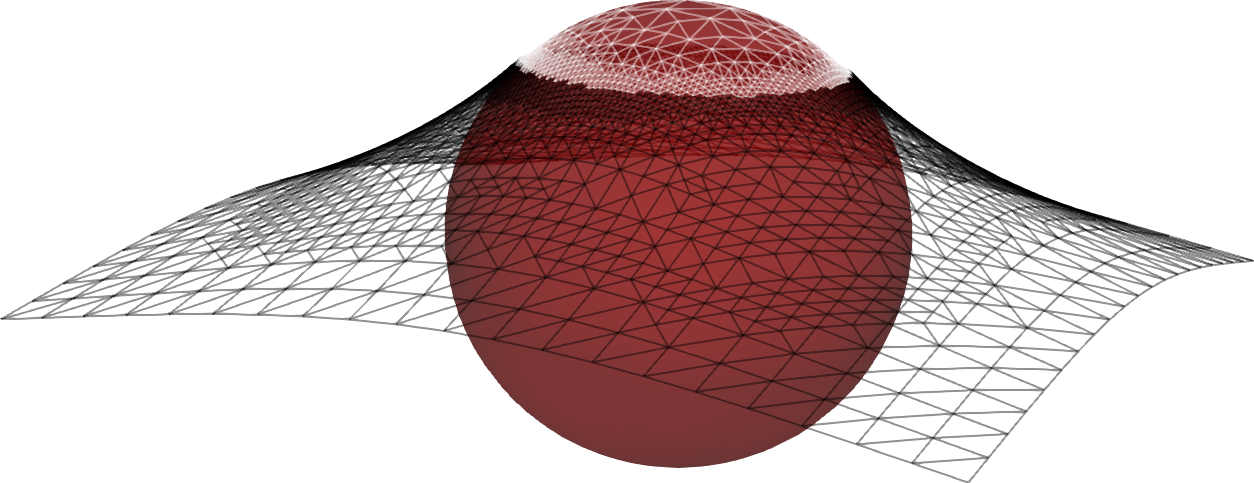
\includegraphics[width=0.8\textwidth]{static/obstacle.png}
\caption{Solution, as wireframe, to a problem with a (hemi)spherical obstacle.}
\label{fig:ball}
\end{figure}

Another physical interpretation of problem \eqref{eq:classical:ncp} is that $u$ models the water pressure, which cannot go below zero ($\psi=0$), in a porous dam \cite[for example]{AinsworthOdenLee1993}.  Section \ref{sec:app} will present another obstacle problem with a highly-nonlinear operator.  In that problem the solution is the surface elevation of a glacier, which is constrained to be above the bedrock (elevation) on which the glacier sits.

As is well-known \cite{KinderlehrerStampacchia1980}, problem \eqref{eq:classical:ncp} has a weak formulation which is a variational inequality (VI) over a Sobolev space.  Let $\cX=H^1(\Omega)$ \cite{ElmanSilvesterWathen2014} and suppose $\psi \in \cX \cap C(\bar\Omega)$.  Let $g:\partial \Omega\to \RR$ be continuous, with $g\ge\psi|_{\partial \Omega}$, and define
\begin{equation} \label{eq:classical:admissible}
\cK = \{u \in \cX \,:\, u \ge \psi \text{ and } u|_{\partial \Omega} = g\}
\end{equation}
as the admissible subset, which is closed and convex in $\cX$.  For $f\in L^2(\Omega)$, the VI formulation of \eqref{eq:classical:ncp} finds $u\in \cK$ so that
\begin{equation} \label{eq:classical:vi}
\int_\Omega \nabla u \cdot \nabla(v - u) \ge \int_\Omega f(v - u) \quad \text{ for all } v \in \cK.
\end{equation}

In Section \ref{sec:vifem} we will recall and extend the theory of such VIs, and their finite element (FE) approximation.  We will generalize from elliptic bilinear forms like \eqref{eq:classical:vi} to coercive nonlinear operators over Banach spaces.  In a conforming FE approximation the numerical solution $u_h$ will solve the same VI weak form, but over a finite-dimensional admissible set constructed on a mesh $\cT_h$.  Similarly to Cea's lemma for PDEs \cite{ElmanSilvesterWathen2014}, the norm errors $\|u-u_h\|$ can be bounded \emph{a priori} by extending the Falk \cite{Falk1974} technique to nonlinear operators, and results in Section \ref{sec:vifem} will show how norm errors are controlled by the approximation properties of the FE space, subject to VI-specific concerns regarding admissibility and the separation of active-set and inactive-set errors.

Adaptive mesh refinement (AMR) uses \emph{a posteriori} information from the numerical solution to strategically add mesh elements to increase the resolution and reduce the numerical error.  For VI problems the simulation goal is often the accurate approximation of the sets in \eqref{eq:classical:sets}.  The attainability of this goal is problem-dependent.

\begin{example} \label{example:notcontinuous}  Suppose $\Omega = (-1,1)$, $\psi(x)=1 - x^2$, and $g(x)=0$, but let $f$ be a constant parameter: $f(x)=\alpha$.  The exact solution $u$ of \eqref{eq:classical:vi} for this data is easily calculated: $u(x)=\psi(x)$ if $\alpha\le 2$ and $u(x)=(\alpha/2)\psi(x)>\psi(x)$ if $\alpha>2$.  Thus for $\alpha \ge 2$ we have $A_u=\Omega$ and $I_u=\emptyset$, while $A_u=\emptyset$ and $I_u=\Omega$ if $\alpha<2$, so the sets \eqref{eq:classical:sets} are not continuous functions of the data $f$ of the problem.  This example can be easily modified to show that, likewise, the sets are not continuous functions of $\psi$ either.
\end{example}

The $\alpha=2$ case of Example \ref{example:notcontinuous} is \emph{degenerate} \cite{KinderlehrerStampacchia1980}, that is, the unconstrained solution happens to match the obstacle on a nonempty open set.  Clearly any predictable convergence results for FE approximations of the solution-dependent sets $A_u,I_u,\Gamma_u$ will depend upon problem nondegeneracy.  Our examples are accordingly non-degenerate.

Furthermore, the effectiveness of different AMR strategies for non-degenerate VI problems depends strongly upon the measure (area or volume) of the active and inactive sets.  This observation motivates the \emph{a posteriori} approaches of this paper.  For example, in certain problems the elements which are significantly interior to the active set require no further computation or refinement.  For such problems, for which examples are given in Sections \ref{sec:results} and \ref{sec:app}, if a solution is desired at higher resolution within the active set, i.e.~where $u=\psi$, then this can be computed in post-processing by arbitrary interpolation of the obstacle data; refinement effort in the active set and during the solution process is wasted.

\begin{example} \label{example:activesets} Examples in Section \ref{sec:results} will cover three 2D classical obstacle problems.  Figure \ref{fig:activesizes} shows their active sets in black.  For the left-hand problem, with a small active set and a long free boundary, our AMR methods refine a large fraction of the elements, namely those close to the free boundary.  The middle problem has a known exact solution; Section \ref{sec:results} shows convergence rates.  For the right-hand problem, a clear performance benefit of our AMR techniques, relative to uniform refinement, comes from avoiding refinement in the active set.  The glaciation application in Section \ref{sec:app} also exploits this efficiency. \end{example}

\begin{figure}[ht]
\noindent \hspace{-1mm} \mbox{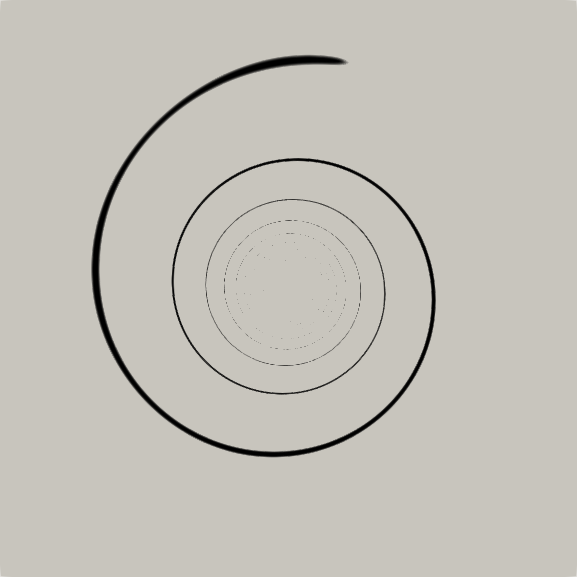
\includegraphics[width=0.32\textwidth]{static/spiral.png} \, 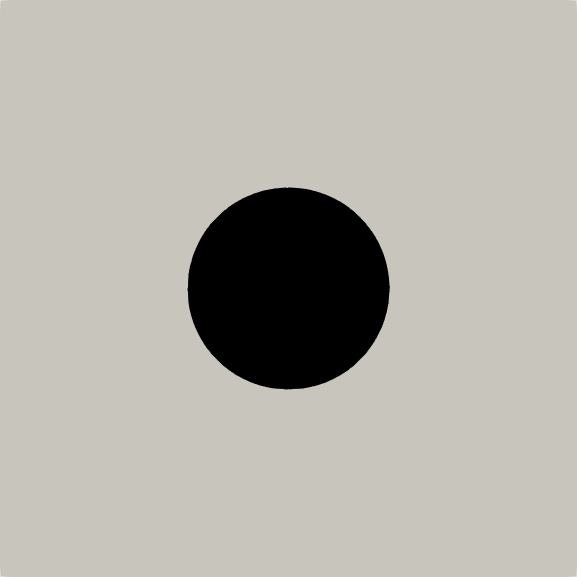
\includegraphics[width=0.32\textwidth]{static/sphere.png} \, 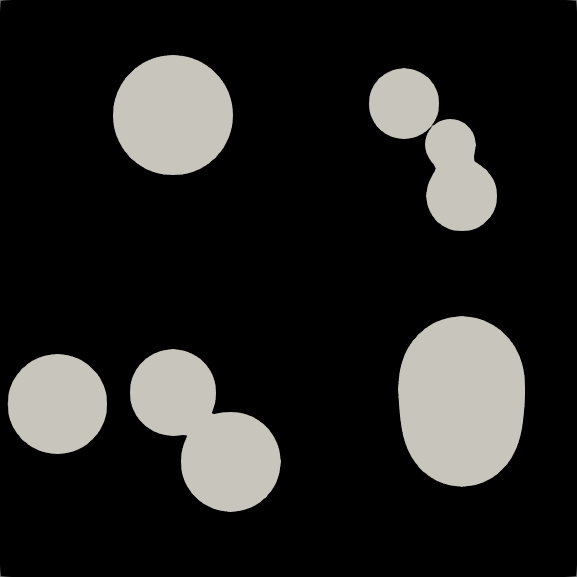
\includegraphics[width=0.32\textwidth]{static/blisters.png}}
\caption{The area (measure) of the active set (black) can vary from small to large (left to right); the middle image matches Figure \ref{fig:ball}.}
\label{fig:activesizes}
\end{figure}

In this work we consider only $P_1$ element spaces over meshs of triangles or tetrahedra, and only $h$-refinement is addressed.  VIs can be solved using $p$-refinement and higher-order elements, but only if nontrivial penalty-type modifications are made to the VI \cite{KeithSurowiec2024}, which is not attempted here.  While the classical obstacle problem \eqref{eq:classical:vi} is equivalent to constrained minimization of a scalar objective, our analysis of FE errors for VI problems does not require such an objective, and our AMR strategies do not exploit one if available.

Three AMR methods for VIs are described in Section \ref{sec:viamr}.  Our implementations use the Firedrake FE library \cite{Rathgeberetal2016} and produce conforming meshes with no hanging nodes.  The first two methods are of tag-and-refine type, only differing by which elements are tagged, with skeleton-based refinement (SBR) \cite{PlazaCarey2000} applied after tagging.  Note that SBR is implemented within PETSc's DMPlex component \cite{petsc-user-ref} and in the Netgen library \cite{Betteridgeetal2024}.  These two methods also require a complementary AMR approach for the PDE problem in the inactive set to achieve convergence; see Section \ref{sec:inactive}.  The third goal-oriented and metric-based method uses the Netgen and Animate \cite{Wallworketal2020} libraries for metric-based mesh adaptation.  Full details are given in Section \ref{sec:viamr}, but here is a high-level view of the methods:

%\renewcommand{\labelenumi}{\emph{\roman{enumi})}}
\begin{itemize}
\item[UDO:] The unstructured dilation operator method discretely identifies elements adjacent to the computed free boundary, employing a graph-based approach to tag neighboring elements for refinement.  It generalizes the image processing operation of dilation \cite{Pratt1991} to unstructured meshes.
\item[VCD:] The variable-coefficient diffusion method starts from a node-wise indicator function for the current computed active set.  This indicator becomes the initial iterate in a single step of a time-dependent heat equation problem, which smooths the indicator about the free boundary.  The smoothed indicator is then thresholded for element tagging (and refinement).
\item[AVM:] The averaged-metric method computes an intermediate representation of the size, shape, and orientation of the new mesh, as a tensor-valued Riemannian metric \cite{Alauzet2010}.  The metric is an average of an anisotropic metric, from the Hessian of the computed solution \cite{Wallworketal2020}, and an isotropic metric, from the diffused active set indicator of the VCD method.  This method approximately maintains mesh complexity, and it adjusts both inactive and active set meshes simultaneously.
\end{itemize}

Example meshes are shown in Figure \ref{fig:threeballmeshes}, generated by 3 levels of refinement using the above three methods, starting from a coarse uniform mesh, on the obstacle problem shown in Figures \ref{fig:activesizes} (middle).  These AMR methods successfully increase the resolution both near the free boundary and where helpful in the inactive set.

% result from examples/sphere.py; note: -n 1 UDO; default VCD; default AVM; theta=0.7 in BR
\begin{figure}[ht]
\noindent \hspace{-1mm} \mbox{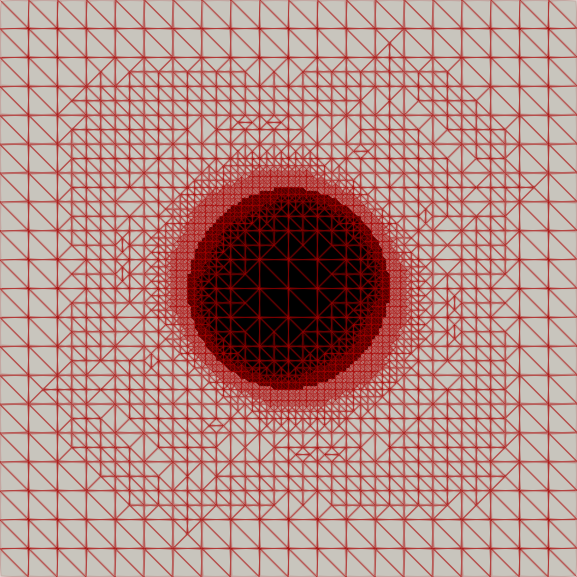
\includegraphics[width=0.32\textwidth]{static/sphereudo.png} \, 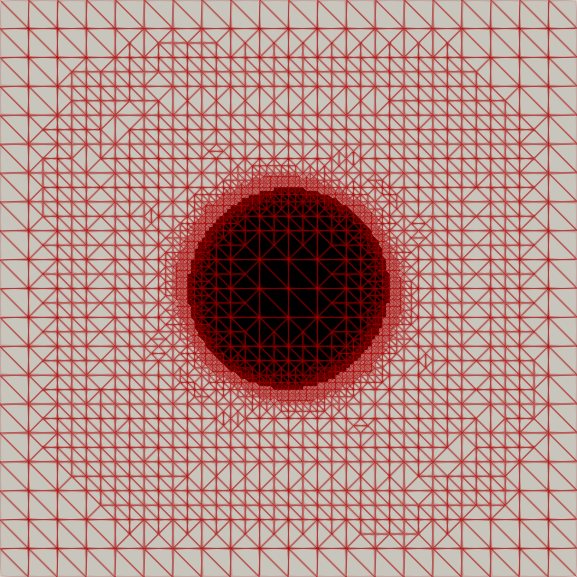
\includegraphics[width=0.32\textwidth]{static/spherevcd.png} \,\,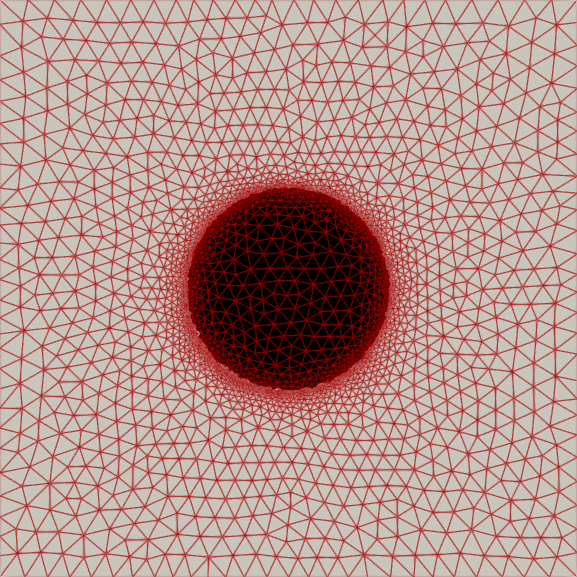
\includegraphics[width=0.32\textwidth]{static/sphereavm.png}}
\caption{Meshes from UDO (left), VCD (middle), and AVM (right) methods.}
\label{fig:threeballmeshes}
\end{figure}

Because the convergence of VI problems is dominated by the error in approximating the free boundary, our AMR schemes quickly concentrate effort around an accurately-computed free boundary, augmented by PDE-type error estimators in the inactive set (Section \ref{sec:inactive}).  This accelerates convergence and reduces unnecessary computation.  Our numerical results in Sections \ref{sec:results} and \ref{sec:app} will justify the somewhat-heuristic nature of our AMR approaches.  

AMR for VI problems has only been lightly explored in the literature.  The first published analysis may be \cite{AinsworthOdenLee1993}, giving an error bound for the classical obstacle problem in terms of local functionals associated with each element.  The monograph by Suttmeier \cite{Suttmeier2008} covers a broader class of problems, including elasticity.  For the classical obstacle problem, the constructable error estimators in these works require heuristic assumptions which may not hold in general.  (See inequality (42) in \cite{AinsworthOdenLee1993}, and the approximation ``$(u-\psi)\lambda_h\approx 0$'' in \cite{Suttmeier2008}.)  To our knowledge these approaches are not found in publicly-available implementations, nor are they as efficient as our strategies for computing high-resolution approximations to free boundaries.

Our focus in this paper is on AMR performance, not solver performance.  We use a fixed, VI-adapted, reduced-space Newton method with line search \cite{BensonMunson2006}, implemented in PETSc \cite{petsc-user-ref}, for all examples.  (Since the constraint $u \geq \psi$ makes VI problems nonlinear, an iterative solver like Newton is required even if the operator is linear.)  Such a numerical method cannot converge quadratically until the active and inactive sets stabilize on the given mesh, equivalently once the discrete free boundary is identified.  Then convergence can occur in one additional iteration, for a linear operator, or otherwise in a few iterations for a well-behaved nonlinear operator.

In summary, here are two principles for the AMR methods of this paper:
\renewcommand{\labelenumi}{\arabic{enumi}.}
\begin{enumerate}
\item Relative to uniform refinement, the methods exhibit significant improvements in convergence rate.  This is measured by norm or free-boundary localization (geometrical) error per mesh degree of freedom (Sections \ref{sec:results} and \ref{sec:app}).
\item Their implementations (\href{https://github.com/StefanoFochesatto/VI-AMR}{{\small \texttt{github.com/StefanoFochesatto/VI-AMR}}}), within the popular Firedrake \cite{Langeetal2016} FE library, are parallel, well-documented, and easy-to-use.
\end{enumerate}

The paper is organized as follows:  Section \ref{sec:vifem} provides \emph{a priori} norm bounds for FE methods applied to VI problems; aspects of this material are new.  Section \ref{sec:inactive} addresses \emph{a posteriori} error estimators which can be applied in the inactive set, and it identifies problems where active-set refinement can be avoided.  Section \ref{sec:viamr} describes the three new AMR methods in more detail.  Sections \ref{sec:results} and \ref{sec:app} compare and discuss their performance on model problems and a realistic glacier application.  Table \ref{tab:abbrev} states the few abbreviations used herein.

\begin{table}[ht]
\centering
\begin{minipage}[t]{0.45\textwidth}
\vspace{0pt}
{\small
\begin{tabular}{ll} \\
AMR       & adaptive mesh refinement \\
AVM$^*$   & averaged-metric \\
BR        & Babu\v{s}ka--Rheinboldt \\
CG        & continuous Galerkin \\
DAG       & directed acyclic graph \\
DG        & discontinuous Galerkin \\
DWR       & dual-weighted residual
\end{tabular}
}
\end{minipage}
\quad
\begin{minipage}[t]{0.45\textwidth}
\vspace{0pt}
{\small
\begin{tabular}{ll} \\
FE        & finite element \\
GR        & gradient recovery \\
PDE       & partial differential equation \\
SBR       & skeleton-based refinement \\
UDO$^*$   & unstructured dilation operator \\
VCD$^*$   & variable-coefficient diffusion \\
VI        & variational inequality
\end{tabular}
}
\end{minipage}
\caption{Abbreviations used in this paper.  Stars indicate the new AMR methods.}
\label{tab:abbrev}
\end{table}


\section{Variational inequalities and their finite element approximations} \label{sec:vifem}

We consider unilateral obstacle problems in Banach spaces.  Let $\Omega \subset \RR^d$, $d=2,3$, be a bounded, polygonal domain.  Let $\cX = W^{1,p}(\Omega)$, $p>1$, be the Sobolev space of measurable functions with $p$th-integrable weak gradients \cite{Evans2010}.  We will assume continuous problem data, with well-defined point values, so suppose $\psi \in \cX \cap C(\bar\Omega)$ and $g\in C(\partial \Omega)$ satisfy $g \ge \psi|_{\partial\Omega}$.  Define the closed and convex admissible subset
\begin{equation} \label{eq:admissible}
\cK = \{v \in \cX \,:\, v \ge \psi \text{ and } v|_{\partial \Omega} = g\} \subset \cX,
\end{equation}
as in \eqref{eq:classical:admissible}.  Observe that generally $\psi\notin\cK$.

Let $\cX'$ be the dual space of $\cX$, and denote the application of $\omega \in \cX'$ to $v\in \cX$ by $\omega[v] \in \RR$.  The norm on $\cX$ is denoted $\|\cdot\|$, and for $\cX'$ the norm is $\|\omega\|' = \sup_{\|v\|=1} |\omega[v]|$.  Let $F:\cK \to \cX'$ be a given operator, generally nonlinear, and let $\ell\in \cX'$ be given.  (While $F$ in Example \ref{example:classicalobstacle} is defined on all of $\cX$, the general operator $F$ might be only defined on $\cK$; Section \ref{sec:app} gives an example.)  The VI associated to this data, a unilateral obstacle problem, is to find $u\in \cK$ so that
\begin{equation} \label{eq:vi}
F(u)[v - u] \ge \ell[v - u] \quad \text{ for all } v \in \cK.
\end{equation}

The VI problems in this paper can be analyzed within the framework of coercivity and Lipschitz continuity.  We say $F$ is $q$-coercive, $1<q<\infty$, if there is $\alpha>0$ so that
\begin{equation} \label{eq:coercive}
(F(v) - F(w))[v - w] \ge \alpha \|v-w\|^q
\end{equation}
for all $v,w \in \cK$.  Note that if $F$ is $q$-coercive then it is also strictly monotone: $(F(v) - F(w))[v - w] > 0$ for $v\ne w$.  Let $B_R(0)$ be the origin-centered open ball in $\cX$ of radius $R>0$.  We say $F$ is Lipschitz on bounded subsets if there is $C(R)>0$ so that
\begin{equation} \label{eq:lipschitz}
\|F(v)-F(w)\|' \le C(R) \|v-w\|
\end{equation}
for all $v,w \in B_R(0)\cap \cK$.  If $F$ satisfies \eqref{eq:lipschitz} then it is continuous.  From coercivity, strict monotonicity, and continuity of $F$ it follows that a unique solution to \eqref{eq:vi} exists \cite[Corollary III.1.8]{KinderlehrerStampacchia1980}.

\begin{example}  \label{example:classicalobstacle}
In the classical obstacle problem \eqref{eq:classical:vi}, over $\cX=H^1(\Omega)=W^{1,2}(\Omega)$, $F(u)[v] = \int_\Omega \grad u\cdot \grad v\,dx$.  This bilinear operator is $2$-coercive because the Laplacian is uniformly elliptic \cite{Evans2010}, and it is Lipschitz over $\cX$ with constant $C=1$.
\end{example}

\begin{example}  \label{example:flatsia}
In glacier model of Section \ref{sec:app}, in the case where the bedrock is flat and the surface mass balance is independent of elevation, the VI problem \eqref{eq:sia:vi} uses a $4$-Laplacian operator over transformed thicknesses $u\in\cX=W^{1,4}(\Omega)$, namely $F(u)[v] = \int_\Omega \Gamma |\grad u|^2\grad u\cdot \grad v\,dx$ where $\Gamma>0$ is constant.  This operator is $4$-coercive \cite[for example]{JouvetBueler2012}, and it is Lipschitz on bounded subsets of $\cX$.  For details see Section \ref{sec:app}.
\end{example}

Note that if the inequality constraint in \eqref{eq:vi} were absent then the residual of the solution $u$ would be zero ($F(u)-\ell=0$); this is the PDE case.  However, for VI \eqref{eq:vi} we only have that $F(u)-\ell=0$ a.e.~within the unknown inactive set $I_u$.  The residual $F(u)-\ell\in \cX'$ might be highly-irregular in the active set $A_u$, but it is nonnegative.  The following lemma states the weak complementarity property associated to VI \eqref{eq:vi}; compare strong-form complementarity \eqref{eq:classical:ncp}.

\begin{lemma} \label{lem:measure}\cite[Theorem II.6.9]{KinderlehrerStampacchia1980}.  Suppose $u\in \cK$ solves \eqref{eq:vi}.  Then $F(u)-\ell=d\mu_u$ is a positive Radon measure supported in the active set $A_u$.  Thus for $w\in\cX$ we have
\begin{equation}
(F(u)-\ell)[w] = \int_{A_u} w\, d\mu_u. \label{eq:measure}
\end{equation}
\end{lemma}

Now let $\cT_h$ be a shape-regular mesh partition (triangulation, etc.) of $\Omega$ \cite{AinsworthOden2000,ElmanSilvesterWathen2014}.  Let $\cX_h \subset \cX \cap C(\bar\Omega)$ be a conforming finite-dimensional FE subspace over $\cT_h$.  Our examples will be piecewise-linear over triangles and tetrahedra: $\cX_h=P_1$.  Assume that there is $g_h\in\cX_h$ such that $g_h=g$ along $\partial \Omega$.  Let $\psi_h \in \cX_h$ be the FE obstacle, which satisfies the compatibility requirement $\psi_h \le g_h$ along $\partial\Omega$; for the moment, $\psi_h$ may be unrelated to $\psi$.  Define the (nonempty) FE admissible set
\begin{equation} \label{eq:fe:admissible}
\cK_h = \{v_h \in \cX_h \,:\, v_h \ge \psi_h \text{ and } v_h|_{\partial \Omega} = g_h|_{\partial\Omega}\}.
\end{equation}
Our FE method seeks $u_h\in\cK_h$ satisfying the VI problem which approximates \eqref{eq:vi}:
\begin{equation} \label{eq:fe:vi}
F(u_h)[v_h - u_h] \ge \ell[v_h - u_h] \quad \text{ for all } v_h \in \cK_h.
\end{equation}
The same argument given for \eqref{eq:vi} shows that this has a unique solution $u_h$.  Define
\begin{equation}
  I_u^h = \{x \in \Omega \,:\, u_h(x) > \psi_h(x)\}, \quad A_u^h = \Omega \setminus I_u^h, \quad \Gamma_u^h = \Omega \cap \partial I_u^h, \label{eq:fe:sets}
\end{equation}
the numerical sets, corresponding to \eqref{eq:classical:sets}, defined \emph{a posteriori} from solving \eqref{eq:fe:vi}.

Because $\cK_h \subset \cX_h \subset \cX$, we might regard \eqref{eq:fe:vi} as a conforming FE method for \eqref{eq:vi}.  However, this is subtle for an obstacle problem as it depends on the relationship between $\psi$ and $\psi_h$.  If $\psi_h$ is an interpolant of $\psi$ then $\cK_h \approx \cK$ in some sense, but one might distinguish three levels of increasingly ``conforming'' admissibility:
\renewcommand{\labelenumi}{\emph{\roman{enumi})}}
\begin{enumerate}
\item $\cK_h \not \subset \cK$
\item $\cK_h \subset \cK$
\item $\cK_h = \cK \cap \cX_h$
\end{enumerate}
Ciarlet \cite[Figure 5.1.3]{Ciarlet2002} observes that situation \emph{i)} generally applies for an interpolated obstacle $\psi_h = \Pi_h \psi$, e.g.~for $\cX_h=P_1$ and when $\psi$ is not convex.  Situation \emph{ii)} holds when $\psi_h \ge \psi$, which can be imposed by using a monotone injection operator, e.g.~``$\psi_h = R^\oplus \psi$'' in the notation from \cite{BuelerFarrell2024}.  (For related ideas, see \cite{GraeserKornhuber2009} and the proof of Theorem 5.1.2 in \cite{Ciarlet2002}.)  The strongest condition \emph{iii)} holds if $\psi_h=\psi$ exactly, for example when $\psi=0$ in the porous dam problems considered by \cite{AinsworthOdenLee1993}.

In any case, the obstacle $\psi$ is given \emph{as data} for VI problem \eqref{eq:vi} over $\cK$.  Point values of $\psi$ can be evaluated as desired to better-represent $u_h$ within the numerical active set $A_u^h$.  That is, over elements where there is active-set correctness, i.e.~$K\in\cT_h$ such that $K \subset A_u \cap A_u^h$, the error $e=u-u_h=\psi-u_h$ can be regarded as zero, or the approximation $\psi_h \approx \psi$ can be improved at will by better interpolation of the data $\psi$ (Section \ref{sec:results}).  As the goal for a refined mesh is to more-accurately solve the FE problem, refinement within a stabilized active set, with a refined and accurate free boundary, is wasted effort.

These ideas already arise in \emph{a priori} bounds for FE error in VI problems.  The following theorem generalizes the Falk bound \cite{Falk1974}; see also \cite[Theorem 5.1.1]{Ciarlet2002}.  It can be extended further to address $F_h\approx F$ \cite[Theorem 6.3]{Bueler2024}, but we will not need such an operator approximation for our examples.

\begin{theorem} \label{thm:genfalk}  For $1<q<\infty$, define the conjugate exponent $q'=q/(q-1)$.  Assume that $F$ is $q$-coercive and Lipschitz on bounded subsets of its domain.  Suppose $u\in\cK$ solves \eqref{eq:vi} and $u_h\in\cK_h$ solves \eqref{eq:fe:vi}.  Let $R_h=\max\{\|u\|,\|u_h\|\}$.  Then there is a constant $c(R_h)>0$, not otherwise depending on $u$ or $u_h$, so that
\begin{align}
\|u-u_h\|^q &\le \frac{2}{\alpha} \bigg( \inf_{v\in\cK} \int_{A_u} (v-u_h)\,d\mu_u + \inf_{v_h\in\cK_h} \int_{A_u} (v_h-\psi)\,d\mu_u  \label{eq:falk} \\
   &\qquad\quad + c(R_h) \inf_{v_h\in\cK_h} \|v_h - u\|^{q'}\bigg). \notag
\end{align}
\end{theorem}

\begin{proof}  For arbitrary $v\in\cK$ and $v_h\in\cK_h$, rewrite \eqref{eq:vi} and \eqref{eq:fe:vi} as $F(u)[u] \le F(u)[v] + \ell[u-v]$ and $F(u_h)[u_h] \le F(u_h)[v_h] + \ell[u_h-v_h]$, respectively.  It follows from these inequalities, and $q$-coercivity of $F$, that
\begin{align}
\alpha \|u-u_h\|^q &\le \left(F(u)-F(u_h)\right)[u-u_h] \label{eq:falkdance} \\
  &= F(u)[u] + F(u_h)[u_h] - F(u)[u_h] - F(u_h)[u] \notag \\
  &\le F(u)[v] + \ell[u-v] + F(u_h)[v_h] + \ell[u_h-v_h] \notag \\
  &\qquad - F(u)[u_h] - F(u_h)[u] \notag \\
  &= F(u)[v-u_h] - \ell[v-u_h] + F(u_h)[v_h-u] - \ell[v_h-u] \notag \\
  &= \left(F(u)-\ell\right)[v-u_h] + \left(F(u)-\ell\right)[v_h-u] \notag \\
  &\qquad + \left(F(u)-F(u_h)\right)[u-v_h] \notag
\end{align}
Since $u,u_h\in B_{R_h} = \{w\in\cX\,:\,\|w\|\le R_h\}$, by the Lipschitz assumption \eqref{eq:lipschitz} there is $C(R_h)>0$ so that the last term from \eqref{eq:falkdance} has bound
\begin{equation}
\left(F(u)-F(u_h)\right)[u-v_h] \le C(R_h) \|u-u_h\|\|u-v_h\|. \label{eq:falklip}
\end{equation}
Now use Young's inequality with $\eps>0$ \cite[Appendix B.2]{Evans2010} on \eqref{eq:falklip}.  We have:
\begin{align}
\alpha \|u-u_h\|^q &\le \left(F(u)-\ell\right)[v-u_h] + \left(F(u)-\ell\right)[v_h-u]  \label{eq:falkyoung} \\
  &\qquad + C(R_h) \left(\eps\|u-u_h\|^q + \tilde C(\eps) \|u-v_h\|^{q'}\right) \notag
\end{align}
where $\tilde C(\eps) = (\eps q)^{-q'/q} {q'}^{-1}$.  Choose $\eps>0$ so that $C(R_h) \eps \le \alpha/2$.  Then
\begin{align}
\frac{\alpha}{2} \|u-u_h\|^q &\le \left(F(u)-\ell\right)[v-u_h] + \left(F(u)-\ell\right)[v_h-u]  \label{eq:falkalmost} \\
  &\qquad + C(R_h) \tilde C(\eps) \|u-v_h\|^{q'} \notag
\end{align}
Apply Lemma \ref{lem:measure} to \eqref{eq:falkalmost}, note $u=\psi$ a.e.~in $A_u$, and take infimums to show \eqref{eq:falk}.\end{proof}

Consider the unconstrained PDE case of \eqref{eq:falk}, namely with $A_u=\emptyset$ and $d\mu_u=0$.  In this case the bound is simply Cea's lemma (quasi-optimality) for $q$-coercive operators, namely $\|u-u_h\| \lesssim \inf_{v_h\in\cK_h} \|v_h - u\|^{1/(q-1)}$.  It is standard in FE theory \cite{AinsworthOden2000,ElmanSilvesterWathen2014} to address the final term in \eqref{eq:falk} by solution regularity and interpolation theory.

If $\psi_h\ge \psi$ then $\cK_h\subset \cK$, and so the first term on the right of \eqref{eq:falk} is zero.  In this case bound \eqref{eq:falk} adds a nonnegative infimum, of an integral over $A_u$, to the above Cea's lemma term.  The addition is large if $v_h\in\cK_h$ is significantly blocked by $\psi_h$ from descending close to the continuum obstacle $\psi$ in the active set $A_u$, and/or if the residual measure $d\mu_u$ is large in $A_u$.

\emph{A priori} error bound \eqref{eq:falk} is further clarified in the $p=2$ and $q=q'=2$ case, i.e.~for the classical obstacle problem.  The bound can then be split between integrals over the (exact) active set and inactive sets.

\begin{corollary} \label{cor:falktwo}
Suppose all the hypotheses of Theorem \ref{thm:genfalk}.  Assume that $p=q=2$, and that $\psi \in C^1(\Omega)$.  Up to constants which depend on $u$ and $u_h$, we may write the \emph{a priori} bound with four integrals,
\begin{subequations}
\label{eq:falktwo}
\begin{align}
\|u-u_h\|^2 \lesssim &\inf_{v\in\cK} \int_{A_u} (v-u_h)\,d\mu_u \label{eq:falktwo:a} \\
&\, + \inf_{v_h\in\cK_h} \int_{A_u} (v_h-\psi)\,d\mu_u \label{eq:falktwo:b} \\
&\, + \inf_{v_h\in\cK_h} \left(\int_{A_u} |\grad v_h - \grad \psi|^2\,dx + \int_{I_u} |\grad v_h - \grad u|^2\,dx\right) \label{eq:falktwo:c}
\end{align}
\end{subequations}
\end{corollary}

\begin{proof}
Apply Poincare's inequality to the final term in \eqref{eq:falk}.
\end{proof}

We now consider bbound \eqref{eq:falktwo} from the point of view of AMR.  The first term \eqref{eq:falktwo:a}, which can be of either sign, is controlled by the choice of $\psi_h$.  Since we are assuming $\cX_h\subset \cX$, this term relates only to discrete admissibility.  This term is zero if $\cK_h \subset \cK$.  The second term \eqref{eq:falktwo:b}, also generally of either sign, relates both to discrete admissibility and to the approximation of $\psi$ using functions from $\cX_h$.  It is nonnegative if $\psi_h\ge \psi$.

Both integrals \eqref{eq:falktwo:a} and \eqref{eq:falktwo:b} are with respect to the residual measure $d\mu_u$, so their size is determined partly by the action of $F$ on the continuum obstacle, and partly by the source term $\ell$.  However, because they are over the active set $A_u$, neither integral \eqref{eq:falktwo:a} nor \eqref{eq:falktwo:b}, nor the $A_u$ integral in \eqref{eq:falktwo:c}, requires mesh refinement so as to improve the quality of the FE solution, \emph{as long as the mesh and solver have accurately located the free boundary}.  Corollary \ref{cor:falktwo} thus suggests why a primary goal of AMR for VIs is to use refinement to generate close approximation $\Gamma_u^h\approx \Gamma_u$.  Computation expended on better approximation of the data $\psi$ in $A_u$, during the solution process, can be avoided if the free boundary is accurately resolved.

These observations are especially easy to exploit within the class of unilateral obstacle problems described in Appendix \ref{app:blistering}.  This class which includes the $\psi=0$ case of the classical obstacle problem \eqref{eq:classical:vi} and the glacier problem of Section \ref{sec:app}.  In such problems one may preprocess the data, marking all the areas where the source term is negative, and then systematically avoid unnecessary active set refinement.

In order for $\Gamma_u^h\approx \Gamma_u$ to be an accurate approximation, the interior condition of the VI, over $I_u$, must be accurately solved, which of course gives the significance of the final integral in \eqref{eq:falktwo:c}.  Our AMR approaches will simultaneously refine near the computed free boundary $\Gamma_u^h$ and in the (computed) inactive set $I_u^h$.


\section{\emph{A posteriori} error estimation in the inactive set} \label{sec:inactive}

For $u\in\cX$ solving VI \eqref{eq:vi}, an interior condition PDE holds in the inactive set $I_u$ \cite{KinderlehrerStampacchia1980}.  Our AMR strategies (Section \ref{sec:viamr}) do \emph{a posteriori} refinement in the geometric vicinity of the free boundary, but they also exploit \emph{a posteriori} error indicators for this interior condition.  We consider two such PDE indicators here.

\begin{example}  \label{example:gradrecovery}  Suppose $\cX_h=\CG_k$ is the continuous, piecewise-polynomial FE space of degree $k$, and consider $u_h\in\cX_h$.  Generally $\grad u_h$ is discontinuous but well-defined on each element.  If $\cY_h=\DG_{k-1}$ denotes the (scalar) discontinuous space with polynomial degree $k-1$ then $\grad u_h \in \cY_h^d$.  Suppose there is a linear operator $G : \cX_h \to \cX_h^d$, called \emph{gradient recovery} (GR) \citep[Chapter 4]{AinsworthOden2000}, so that $G(u_h)\approx \grad u$ in some sense, assuming of course that $u_h\approx u$ in $\cX$.  Then, over an element $K \in\cT_h$, the error indicator $\eta_K\ge 0$ for this GR method is
\begin{equation} \label{eq:gradrecoveryindicator}
\eta_K^2 = \int_K \left|G(u_h) - \grad u_h\right|^2.
\end{equation}
We also define $\eta^2 = \sum_{K\in\cT_h} \eta_K^2$.
\end{example}

Generally one applies the indicator to a solution $u_h \in \cK_h$ of \eqref{eq:fe:vi}, but formula \eqref{eq:gradrecoveryindicator} is well-defined for any $u_h \in \cX_h$.  For certain gradient recovery methods $G$ applied to the Poisson equation, $\eta \sim |u-u_h|_{H^1}$ (energy norm) as $h\to 0$ \cite[Theorem 4.4]{AinsworthOden2000}.

Our application of GR in Section \ref{sec:app} will simply use orthogonal projection in $L^2$.  That is, $w = G(u_h) \in \cX_h^d$ is defined to be the minimizer of
\begin{equation} \label{eq:gradrecoveryprojection}
J(w) = \int_\Omega |w - \grad u_h|^2\,dx.
\end{equation}
In this application $\cX_h = \CG_1$, thus $\grad u_h$ is in (vector-valued) $\DG_0$.

The second indicator, applied in Section \ref{sec:results} to the Poisson equation interior condition of classical problem \eqref{eq:classical:vi}, is a well-known \emph{explicit error estimator} \cite[Chapter 2]{AinsworthOden2000}.

\begin{example}  \label{example:br}  Suppose $u \in H^1(\Omega)$ solves the weak form Poisson equation $a(u,v) = \int_\Omega f v\,dx$ for all $v \in H^1_0(\Omega)$, with $u=g$ on $\partial \Omega$, for $a(u,v)=\int_\Omega \grad u\cdot \grad v\,dx$.  Suppose that $u_h\in\cX_h=\CG_1$ solves the corresponding finite-dimensional weak form.  For each element $K \in \cT_h$, define $n_K$ as the unit outward normal vector on $\partial K$.  For a pair of elements $L,K$ incident to an edge $\gamma$, and any vector field $Z$ with traces $Z_L,Z_K$ on $\gamma$, let $\left\llbracket Z \cdot n \right\rrbracket = Z_L \cdot n_L + Z_K \cdot n_K$ be the jump of $Z$ on $\gamma$.  Given the (strong) residual $r(u_h)=-\nabla^2 u_h - f$ of the Poisson equation, well-defined within an element $K$, the Babu\v{s}ka--Rheinboldt (BR) \cite{BabuskaRheinboldt1979} error estimator is
\begin{equation} \label{eq:brestimator}
\eta_K^2 = h_K^2 \int_K |r(u_h)|^2\,dx + \frac{h_K}{2} \sum_{\gamma \in \partial K \setminus \partial \Omega} \int_{\gamma} \left\llbracket \grad u_h \cdot n \right\rrbracket^2\,dS,
\end{equation}
where $h_K$ is the diameter of $K$.  It can be shown \cite[Chapter 2]{AinsworthOden2000} that the energy error is bounded by $\eta^2 = \sum_{K\in\cT_h} \eta_K^2$:
\begin{equation} \label{eq:brbound}
|u-u_h|_{H^1}^2 = \int_\Omega |\grad(u-u_h)|^2\,dx \le C \eta^2.
\end{equation}
Similarly the $L^2$ error can be bounded by an estimator, one which replaces the powers in \eqref{eq:brestimator} by $h_K^4,h_K^3$, respectively \cite[Section 2.4]{AinsworthOden2000}.
\end{example}

For the results in Sections \ref{sec:results} and \ref{sec:app}, whether $\eta_K$ is computed as in Example \ref{example:gradrecovery} or \ref{example:br}, we will treat the values $\eta_k$ as local element-wise error estimators.  The set $\{\eta_K\}$ will be thresholded to providing tagging of elements for refinement; see \cite[Section 4.2]{BangerthRannacher2003} for discussion of such techniques.  Specifically, all (computed) inactive elements satisfying $\eta_K \ge \theta \max \eta_K$, for $0<\theta<1$, will be tagged and refined.

The BR error estimator is explicit and easily-computed.  Ainsworth, Oden, and Lee \cite{AinsworthOdenLee1993} extend it to certain obstacle problems, but with heuristic aspects.  On the other hand, for certain PDE problems, alternative estimators are provided by the \emph{dual weighted residual} (DWR) technique \cite{BangerthRannacher2003}.  These are defined using a particular quantity of interest and some approximately-computed nonlocal weights, essentially Green's functions of the adjoint PDE.  Suttmeier \cite{Suttmeier2008} has extended this DWR technique to certain VI problems, but this also requires heuristic steps even for the classical obstacle problem.  In this paper we avoid the complexity of the techniques in \cite{AinsworthOdenLee1993} and \cite{Suttmeier2008}, and instead take a more pragmatic approach.  In the next Section we propose fast, and again heuristic, refinement near a computed free boundary, combined with application of a gradient-recovery or BR estimator within the computed inactive sets.


\section{New adaptive mesh refinement strategies} \label{sec:viamr}

Our first two methods for adaptive mesh refinement (AMR) for VIs, Algorithms \ref{alg:udo} and \ref{alg:vcd}, are of \emph{tag-and-refine} type, with targeted refinement near the free boundary.  A third, more-expensive \emph{metric-based mesh adaptation} approach \cite{Wallworketal2020} follows; Algorithm \ref{alg:avm} can hold the mesh complexity approximately constant.  These methods all start from a computed solution to FE VI problem \eqref{eq:fe:vi}.  We need only the mesh $\cT_h$, the obstacle $\psi_h \in \cX_h$, and the admissible solution $u_h \in \cK_h \subset \cX_h$.  The following two concepts are fundamental.

\begin{definition} \label{def:nodalactive}
Denote the vertices of $\cT_h$ by $x_j$.  Given $u_h \ge \psi_h$ and a tolerance $\text{tol}>0$, the \emph{nodal active set indicator} is the unique $\nu_h\in\cX_h$ satisfying
	$$\nu_h(x_j) = \begin{cases} 1, & u_h(x_j) - \psi_h(x_j) < \text{tol} \\
	                             0, & \text{otherwise.}\end{cases}$$
\end{definition}

\begin{definition} \label{def:marking}
An \emph{element marking} of $\cT_h$ is a piecewise-constant indicator function $\oneh \in \DG_0(\cT_h)$ with values in $\{0,1\}$.
\end{definition}

For PDE problems, an element marking is typically derived from an error estimator $\eta_K$ associated with a quantity of interest, such as energy or $L^2$ norm error, or a local functional \cite{BangerthRannacher2003}; we gave examples in Section \ref{sec:inactive}.  However, a primary quantity of interest for obstacle problems is \emph{vicinity to the unknown free boundary}.  We do not associate this concept with a precise functional.  Instead Algorithms \ref{alg:udo} and \ref{alg:vcd} proceed heuristically to convert a nodal active set indicator $\nu_h$ (Definition \ref{def:nodalactive}) into an element marking $\oneh$ (Definition \ref{def:marking}), with the goal of improving the approximation of the free boundary.

The use of PETSc DMPlex queries is essential to Algorithm \ref{alg:udo} below, so let us sketch how this class supports unstructured meshes \cite{Langeetal2016}.  A DMPlex object stores the topology (connectivity) of a dimension $d=1,2,3$ mesh.  Every mesh entity, regardless of dimension, is assigned a unique index.  Mesh connectivity is understood as a stratified directed acyclic graph (DAG), in which a covering/incidence relationship between mesh entities determines the directed edges.  For example, a triangle within a 2D mesh is covered by its three edges, which are covered by their two endpoints (vertices).  Each stratum (``height'') in the DAG represents a dimensional class of mesh entity, thus the cells, edges, and vertices in a 2D mesh are at heights $0$, $1$, $2$.  Given the index $p$ of a mesh entity, the basic DMPlex mesh topology queries \cite{petsc-user-ref} are $\text{\emph{cone}}(p)$, the set of indices of entities which cover entity $p$, and its dual $\text{\emph{support}}(p)$, the set of entities which are covered by $p$.  The transitive closure of \emph{cone} is $\text{\emph{closure}}(p)$, and that of \emph{support} is $\text{\emph{star}}(p)$.  In our application we need only the vertices in the element closure; we denote this as $\text{\emph{closure}}^\wedge(k)$.  Similarly, $\text{\emph{star}}_\vee(j)$ extracts only elements in the star of vertex $x_j$.

The Unstructured Dilation Operator (UDO) method, Algorithm \ref{alg:udo}, first computes a nodal active set indicator $\nu_h$ from $u_h$.  Denoting the degrees of freedom in $\DG_0(\cT_h)$ by $x_k$, it finds the set of indices $k$ of elements such that $0<\nu_h(x_k)<1$.  If $u_h \in \CG_1$ then this condition holds when the element is incident to both active and inactive vertices.  Then the method alternates closure and star on the element set $n$ times, expanding the marking by $n$ element layers, to generate an element marking $\oneh$.

\begin{algorithm}[ht]
	\caption{Unstructured Dilation Operator (UDO) element marking}
	\begin{algorithmic}[1]
		\Require mesh $\cT_h$, solution $u_h \in \cK_h$, obstacle $\psi_h \in \cX_h$, tolerance $\text{tol} > 0$, and expansion parameter $n\ge 1$.
		\State Compute nodal active set indicator $\nu_h \in \cX_h$ for $u_h$.
		\State Find initial element index set $S_0$: \,$k\in S_0$ if $\nu_h(x_k) \in (0,1)$.
		\For{$i=0,\dots,n-1$}
		    $$S_{i+1} = \bigcup_{k\in S_i}\, \bigcup_{j\in \text{\emph{closure}}^\wedge(k)} \text{\emph{star}}_\vee(j)$$
		\EndFor \\
		\Return marking $\oneh \in \DG_0(\cT_h)$ of all elements with indices in $S_n$.
	\end{algorithmic}
\label{alg:udo}
\end{algorithm}

The main motivation of the UDO method is that if the approximation $u_h\approx u$ is good for a non-degenerate VI problem \eqref{eq:vi} then the free boundary $\Gamma_u$ should pass through, or close to, the elements indicated \emph{a posteriori} by $\oneh$.  Indeed, in the results Sections \ref{sec:results} and \ref{sec:app} we only consider $n=1$ and $n=2$, as this much expansion seems to suffice for accurate representation of the free boundary under a few refinements.

While the UDO strategy explicitly manipulates indices, our second strategy, called Variable Coefficient Diffusion (VCD) and shown in Algorithm \ref{alg:vcd}, is a smoothed approximation of UDO based on continuum ideas.  Again it generates a marking $\oneh$ for elements near the computed free boundary, and again the first step is to compute a nodal active set indicator $\nu_h \in \CG_1$.  However, in VCD this function is used as the initial condition of a time-dependent, variable-coefficient diffusion equation,
\begin{equation} \label{eq:diffusioneqn}
\frac{\partial s}{\partial t} = \Div\left(D \grad s\right), \qquad s(t=0) = \nu_h,
\end{equation}
with Neumann (natural) boundary conditions, a well-posed problem.  A solution of \eqref{eq:diffusioneqn} at any $t>0$ is a smoothed form of $\nu_h$.  The diffusivity here is set to the square of the element diameter $h(k)$, namely $D=C h(k)^2$ with $C=0.5$ by default; note that $h(k)$ varies over the mesh.  The diffusion range is thus proportional to the element diameter everywhere along the free boundary.  In fact \eqref{eq:diffusioneqn} is not solved exactly, or even very accurately, as we only compute $s_h\in\cX_h$ from a single backward-Euler step of duration $\Delta t = 1$.  The default solver for this linear and elliptic problem is four iterations of conjugate gradient, preconditioned by incomplete-Cholesky factorization \cite{Bueler2021}.  This inexpensive approximate solver has linear complexity in the vertices.

\begin{algorithm}[ht]
	\caption{Variable Coefficient Diffusion (VCD) element marking}
	\begin{algorithmic}[1]
		\Require mesh $\cT_h$, solution $u_h \in \cK_h$, obstacle $\psi_h \in \cX_h$, tolerance $\text{tol} > 0$, coefficient $C>0$, and threshold interval $0 < \alpha < \beta < 1$.
		\State Compute nodal active set indicator $\nu_h \in \cX_h$ for $u_h$.
		\State For $h$ the element diameter, let $D=C h^2 \in \DG_0(\cT_h)$.
		\State Approximately solve for $s_h\in\cX_h$, with Neumann boundary conditions:
		  $$s_h - \Div(D \grad s_h) = \nu_h$$ \\
		\Return marking $\oneh \in \DG_0(\cT_h)$ of all elements such that $s_h(x_k) \in (\alpha,\beta)$.
    \end{algorithmic}
\label{alg:vcd}
\end{algorithm}

Figure \ref{fig:vcdillustration} illustrates how the VCD algorithm applies to a one-dimensional obstacle problem.  Note that there are parameters to consider with this technique, especially the thresholds $\alpha$ and $\beta$, with defaults $\alpha=0.2$ and $\beta=0.8$.  Lowering $\alpha$ toward zero increases resolution in the inactive set near the (computed) free boundary, while increasing $\beta$ toward one increases resolution on the active set side.

\begin{figure}[ht]
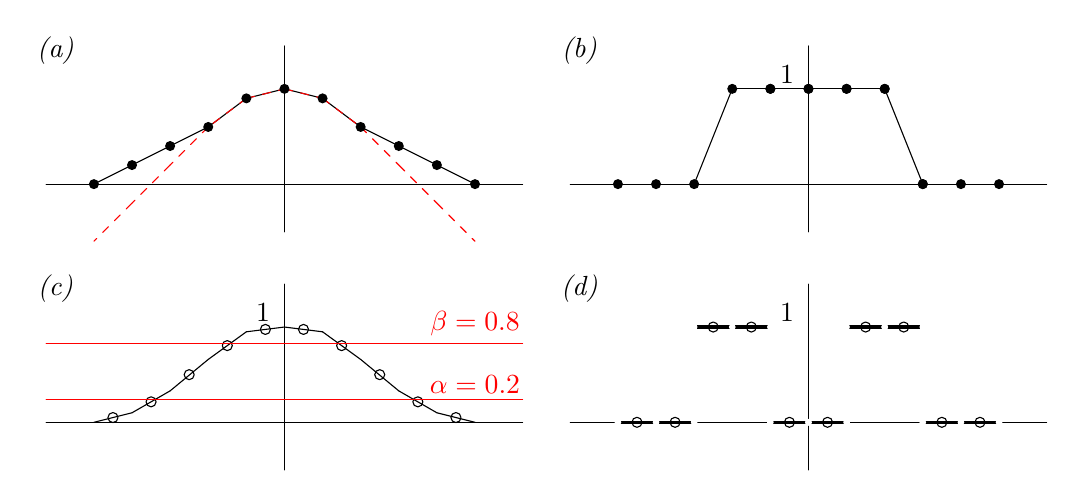
\begin{tikzpicture}[line cap=round,line join=round,>=triangle 45,scale=1.21]

%%%%%% (a) %%%%%
    \draw (0.4,0.9) -- (0.8,0.6);
    \draw (0.8,0.6) -- (1.2,0.4);
    \draw (1.2,0.4) -- (1.6,0.2);
    \draw (-0.4,0.9) -- (-0.8,0.6);
    \draw (-0.8,0.6) -- (-1.2,0.4);
    \draw (-1.2,0.4) -- (-1.6,0.2);
    \draw (-1.6,0.2) -- (-2,0);
    \draw (1.6,0.2) -- (2,0);
    \draw (-0.4,0.9) -- (0,1);
    \draw (0,1) -- (0.4,0.9);

    % New red curve aligning with black nodes
    \draw[red,dashed] (1.6,-.2) -- (2,-.6);
    \draw[red,dashed] (1.2,0.2) -- (1.6,-.2);
    \draw[red,dashed] (0.8,0.6) -- (1.2,0.2);
    \draw[red,dashed] (0.4,0.9) -- (0.8,0.6);
    \draw[red,dashed] (0,1) -- (0.4,0.9);
    \draw[red,dashed] (-0.4,0.9) -- (0,1);
    \draw[red,dashed] (-0.4,0.9) -- (-0.8,0.6);
    \draw[red,dashed] (-0.8,0.6) -- (-1.2,.2);
    \draw[red,dashed] (-1.2, .2) -- (-1.6,-.2);
    \draw[red,dashed] (-1.6,-.2) -- (-2,-.6);

    \begin{scriptsize}
      \fill [color=black] (-0.4,0.9) circle (1.5pt);
      \fill [color=black] (0.4,0.9) circle (1.5pt);
      \fill [color=black] (0.8,0.6) circle (1.5pt);
      \fill [color=black] (1.2,0.4) circle (1.5pt);
      \fill [color=black] (1.6,0.2) circle (1.5pt);
      \fill [color=black] (-0.8,0.6) circle (1.5pt);
      \fill [color=black] (-1.2,0.4) circle (1.5pt);
      \fill [color=black] (-1.6,0.2) circle (1.5pt);
      \fill [color=black] (-2,0) circle (1.5pt);
      \fill [color=black] (2,0) circle (1.5pt);
      \fill [color=black] (0,1) circle (1.5pt);
    \end{scriptsize}

    % Add Axes
    \draw[-] (-2.5,0) -- (2.5,0); % x-axis
    \draw[-] (0,-0.5) -- (0,1.45); % y-axis

    \node at (-2.4,1.4) {\emph{(a)}};


%%%%%% (b) %%%%%
\begin{scope}[shift={(5.5,0.0)}]
    \draw (1.6,0) -- (2,0);
    \draw (1.2,0) -- (1.6,0);
    \draw (0.8,1) -- (1.2,0);
    \draw (0.4,1) -- (0.8,1);
    \draw (0,1) -- (0.4,1);
    \draw (-0.4,1) -- (0,1);
    \draw (-0.4,1) -- (-0.8,1);
    \draw (-0.8,1) -- (-1.2,0);
    \draw (-1.2,0) -- (-1.6,0);
    \draw (-1.6,0) -- (-2,0);

    % Add black vertices
    \begin{scriptsize}
      \fill [color=black] (1.6,0) circle (1.5pt);
      \fill [color=black] (2,0) circle (1.5pt);
      \fill [color=black] (1.2,0) circle (1.5pt);
      \fill [color=black] (0.8,1) circle (1.5pt);
      \fill [color=black] (1.2,0) circle (1.5pt);
      \fill [color=black] (0.4,1) circle (1.5pt);
      \fill [color=black] (0.8,1) circle (1.5pt);
      \fill [color=black] (0,1) circle (1.5pt);
      \fill [color=black] (0.4,1) circle (1.5pt);
      \fill [color=black] (-0.4,1) circle (1.5pt);
      \fill [color=black] (0,1) circle (1.5pt);
      \fill [color=black] (-0.4,1) circle (1.5pt);
      \fill [color=black] (-0.8,1) circle (1.5pt);
      \fill [color=black] (-1.2,0) circle (1.5pt);
      \fill [color=black] (-1.6,0) circle (1.5pt);
      \fill [color=black] (-2,0) circle (1.5pt);
    \end{scriptsize}
    
    % Add Axes
    \draw[-] (-2.5,0) -- (2.5,0); % x-axis
    \draw[-] (0,-0.5) -- (0,1.45); % y-axis

    % Label y=1
    \node at (-0.05,1.15) [left] {1};

    \node at (-2.4,1.4) {\emph{(b)}};
\end{scope}


%%%%%% (c) %%%%%
\begin{scope}[shift={(0.0,-2.5)}]
    % Draw the smoothed curve
    \draw (1.6, 0.1) -- (2,0);      
    \draw (1.2, 0.33) -- (1.6, 0.1);
    \draw (0.8, 0.66) -- (1.2, 0.33);
    \draw (0.4, 0.95) -- (0.8, 0.66);
    \draw (0,1) -- (0.4, 0.95);
    \draw (-0.4, 0.95) -- (0,1);
    \draw (-0.4, 0.95) -- (-0.8, 0.66);
    \draw (-0.8, 0.66) -- (-1.2, 0.33);
    \draw (-1.2, 0.33) -- (-1.6, 0.1);
    \draw (-1.6, 0.1) -- (-2,0);

    % Add black circles at element centers
    \begin{scriptsize}
      \draw [color=black] (1.8, 0.05) circle (1.5pt);
      \draw [color=black] (1.4, 0.215) circle (1.5pt);
      \draw [color=black] (1.0, 0.5) circle (1.5pt);
      \draw [color=black] (0.6, 0.805) circle (1.5pt);
      \draw [color=black] (0.2, 0.975) circle (1.5pt);
      \draw [color=black] (-0.2, 0.975) circle (1.5pt);
      \draw [color=black] (-0.6, 0.805) circle (1.5pt);
      \draw [color=black] (-1.0, 0.5) circle (1.5pt);
      \draw [color=black] (-1.4, 0.215) circle (1.5pt);
      \draw [color=black] (-1.8, 0.05) circle (1.5pt);
    \end{scriptsize}

    % Add Axes
    \draw[-] (-2.5,0) -- (2.5,0); % x-axis
    \draw[-] (0,-0.5) -- (0,1.45); % y-axis

    % Label y=1
    \node at (-0.05,1.15) [left] {1};

    % Add red horizontal lines; pretend heights are 0.8 and 0.2
    \draw[red] (-2.5, 0.83) -- (2.5, 0.83);
    \draw[red] (-2.5, 0.24) -- (2.5, 0.24);
    % Label the heights of the red lines
    \node[red] at (2, 0.8) [above] {$\beta=0.8$};
    \node[red] at (2, 0.2) [above] {$\alpha=0.2$};

    \node at (-2.4,1.4) {\emph{(c)}};
\end{scope}


%%%%%% (d) %%%%%
\begin{scope}[shift={(5.5,-2.5)}]

    \draw[very thick] (1.6,0) -- (2,0);      
    \draw[very thick] (1.2,0) -- (1.6,0);
    \draw[very thick] (0.8,1) -- (1.2,1);
    \draw[very thick] (0.4,1) -- (0.8,1);
    \draw[very thick] (0,0) -- (0.4,0);
    \draw[very thick] (-0.4,0) -- (0,0);
    \draw[very thick] (-0.4,1) -- (-0.8,1);
    \draw[very thick] (-0.8,1) -- (-1.2,1);
    \draw[very thick] (-1.2,0) -- (-1.6,0);
    \draw[very thick] (-1.6,0) -- (-2,0);

    % Add Axes
    \draw[-] (-2.5,0) -- (2.5,0); % x-axis
    \draw[-] (0,-0.5) -- (0,1.45); % y-axis

    % Label y=1
    \node at (-0.05,1.15) [left] {1};

    % Add Nodes in white to separate elements
    \begin{scriptsize}
    \fill [color=white] (1.6,0) circle (1.0pt);
    \fill [color=white] (2,0) circle (1.0pt);      
    \fill [color=white] (1.2,0) circle (1.0pt);
    \fill [color=white] (0.8,1) circle (1.0pt);
    \fill [color=white] (1.2,1) circle (1.0pt);
    \fill [color=white] (0.4,1) circle (1.0pt);
    \fill [color=white] (0.8,1) circle (1.0pt);
    \fill [color=white] (0,0) circle (1.0pt);
    \fill [color=white] (0.4,0) circle (1.0pt);
    \fill [color=white] (-0.4,0) circle (1.0pt);
    \fill [color=white] (0,0) circle (1.0pt);
    \fill [color=white] (-0.4,1) circle (1.0pt);
    \fill [color=white] (-0.8,1) circle (1.0pt);
    \fill [color=white] (-1.2,1) circle (1.0pt);
    \fill [color=white] (-1.2,0) circle (1.0pt);
    \fill [color=white] (-1.6,0) circle (1.0pt);
    \fill [color=white] (-2,0) circle (1.0pt);
    \end{scriptsize}

    % Add black circles at element centers
    \begin{scriptsize}
      \draw [color=black] (1.8, 0.0) circle (1.5pt);
      \draw [color=black] (1.4, 0.0) circle (1.5pt);
      \draw [color=black] (1.0, 1.0) circle (1.5pt);
      \draw [color=black] (0.6, 1.0) circle (1.5pt);
      \draw [color=black] (0.2, 0.0) circle (1.5pt);
      \draw [color=black] (-0.2, 0.0) circle (1.5pt);
      \draw [color=black] (-0.6, 1.0) circle (1.5pt);
      \draw [color=black] (-1.0, 1.0) circle (1.5pt);
      \draw [color=black] (-1.4, 0.0) circle (1.5pt);
      \draw [color=black] (-1.8, 0.0) circle (1.5pt);
    \end{scriptsize}

    \node at (-2.4,1.4) {\emph{(d)}};
\end{scope}

\end{tikzpicture}
  
\caption{Illustration of VCD: \emph{(a)} The function $u_h$ (solid) is an approximate solution to \eqref{eq:fe:vi}, with nodes $x_j$ shown (solid dots), and obstacle $\psi_h$ (red dashed).  \emph{(b)} Nodal active set indicator $\nu_h \in \CG_1(\cT_h)$, with values in $\{0,1\}$.  \emph{(c)} Smoothed indicator $s_h$, with element degrees of freedom $x_k$ shown (circles) and thresholding levels (red).  \emph{(d)} Element marking $\oneh$; 4 elements are marked for refinement.}
\label{fig:vcdillustration}
\end{figure}

It turns out to be helpful, especially when solving highly-nonlinear obstacle problems like that in Section \ref{sec:app}, to have the user of Algorithms \ref{alg:udo} and \ref{alg:vcd} also set a minimum element diameter $\hmin$.  To implement this bound, after running these Algorithms we (un)set the indicator for element $K$, i.e.~$\oneh|_K=0$, for any element with $h_K < \hmin$.

From the marking $\oneh$, computed by either Algorithm, we then apply \emph{skeleton-based refinement} (SBR) \cite{PlazaCarey2000} to generate a refined mesh with good mesh quality.  Elements with $\oneh=1$ are refined, as are other elements so as to avoid hanging nodes.  Two implementations of SBR are available to Firedrake applications, from PETSc DMPlex \cite{petsc-user-ref} and the Netgen library \cite{Betteridgeetal2024}, but only the latter is currently capable of 3D refinement.

Our third AMR method, called \emph{averaged-metric} (AVM; Algorithm \ref{alg:avm}), uses metric-based mesh adaptation \cite{Alauzet2010}.  Instead of marking elements for refinement, mesh adaptation generates a wholely new mesh matching resolution and complexity targets.  Adaptation is driven by an \emph{a posteriori} computed metric field, defined as a continuous, matrix-valued function $M_h:\Omega \to \RR^{d\times d}$ with each value $M_h(x)$ a symmetric and positive-definite matrix.  Such a metric contains local information on distances, areas, and volumes \cite{LoseilleAlauzet2011}.  From the metric the mesher itself generates a unit mesh \cite{Alauzet2010}.  The refined mesh has variable and anisotropic edge lengths in the original space.

AVM again starts from $u_h$ and $\psi_h$.  The first metric is isotropic, and it is computed from the gradient of a smoothed nodal active set indicator, namely $s_h$ from the VCD method (Algorithm \ref{alg:vcd}).  The second metric is anisotropic, computed as an approximate Hessian of $u_h$ via a Hessian-recovery technique \cite{Alauzet2010}.  The absolute value of the Hessian is used, which well-defined for a symmetric matrix \cite{Wallworketal2020}.  These metrics are in the matrix-valued $\CG_1$ FE space, with metric normalization constants computed from target complexity and element diameter bounds in a standard manner \cite{Wallworketal2020}.  By construction, the first metric should generate small elements near the free boundary, while the second should reduce FE approximation error, specifically in the inactive set, according to the standard interpolation theory \cite{Ciarlet2002}.  The final metric is a weighted average of the two earlier metrics.  Note that the final metric is anisotropic and free-boundary aware, but it implies refinement in both the active and inactive sets.  Our implementation calls the Animate library (\href{https://github.com/mesh-adaptation/animate}{{\small \texttt{github.com/mesh-adaptation/animate}}}) to construct, normalize, and average the metrics, and the Pragmatic library \cite{Gormanetal2012} for metric-based meshing.

\begin{algorithm}[ht]
	\caption{Averaged-metric (AVM) mesh adaptation}
	\begin{algorithmic}[1]
		\Require mesh $\cT_h$, solution $u_h \in \cK_h$, obstacle $\psi_h \in \cX_h$, target complexity $N$, element diameter bounds $0<\hmin<\hmax$, and averaging parameter $0\le \gamma \le 1$
		\State Compute $s_h \in \cX_h$ from Algorithm \ref{alg:vcd}, using $u_h$ and $\psi_h$.
		\State Compute normalized isotropic free-boundary metric: $M_1(x)=c_1 |\grad s_h(x)| I_{d\times d}$.
		\State Compute normalized anisotropic metric from Hessian: $M_2(x)=c_2 |H u_h(x)|$.
		\State Average the metrics: $M(x) = \gamma M_1(x) + (1-\gamma) M_2(x)$. \\
		\Return new mesh $\tilde \cT_h$ which is unit with respect to $M(x)$.
    \end{algorithmic}
\label{alg:avm}
\end{algorithm}

The right-hand image in Figure \ref{fig:threeballmeshes}, in the Introduction, shows an AVM result on the ``ball'' obstacle problem (Figure \ref{fig:activesizes}, middle).  Note that iterating the AVM method, even while holding the target mesh complexity constant, can be worthwhile because the increased resolution near the free boundary allows the \emph{a posteriori} metric to become more effective.  However, because of the many nontrivial computations in metric-based methods \cite{Alauzet2010,Wallworketal2020}, one AVM iteration is notably more expensive than an iteration of UDO or VCD; see Section \ref{sec:results}.

All three methods, UDO, VCD, and AVM, run in parallel under the MPI protocol used by Firedrake \cite{Langeetal2016} and PETSc.  However, only UDO produces results which are independent of the number of processes.  The VCD method can be configured to have this property by choosing a direct solver for problem \eqref{eq:diffusioneqn}, but this reduces scalability.  The preconditioned Krylov solver is preferred for VCD performance, although its default parallel block preconditioner is slightly-dependent on process count \cite{Bueler2021}.

We end this section with two basic Python examples which illustrate how to use the open source VIAMR library (\href{https://github.com/StefanoFochesatto/VI-AMR}{{\small \texttt{github.com/StefanoFochesatto/VI-AMR}}}).

\begin{example} \label{example:AOL}
Consider now Example 1 from \cite{AinsworthOdenLee1993}, a classical obstacle problem over a rectangle, with obstacle $\psi=0$ and a known exact solution.  The complete code below applies the Firedrake and VIAMR libraries to solve this problem.  First it generates a uniform coarse mesh, then it applies VCD marking for the free boundary, and then it refines to a new mesh (Figure \ref{fig:resultAOL}).  For this example there is no refinement in the inactive set, but that would be necessary for convergence; compare the next Section.
\inputminted[linenos, frame=lines]{python}{../examples/aol.py}
\end{example}

\begin{figure}[ht]
\centering
\mbox{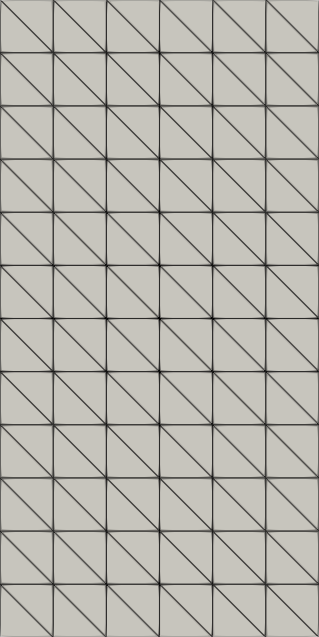
\includegraphics[width=0.19\textwidth]{static/aol-mesh.png} \qquad\qquad
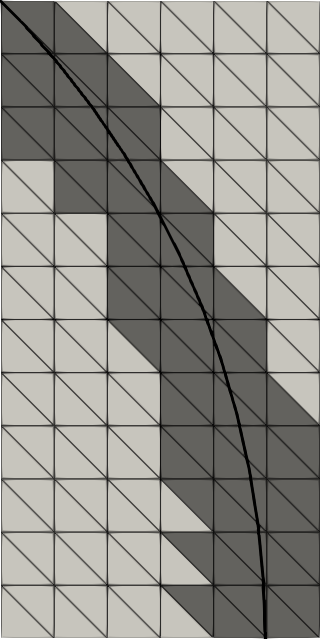
\includegraphics[width=0.19\textwidth]{static/aol-marked.png} \qquad\qquad
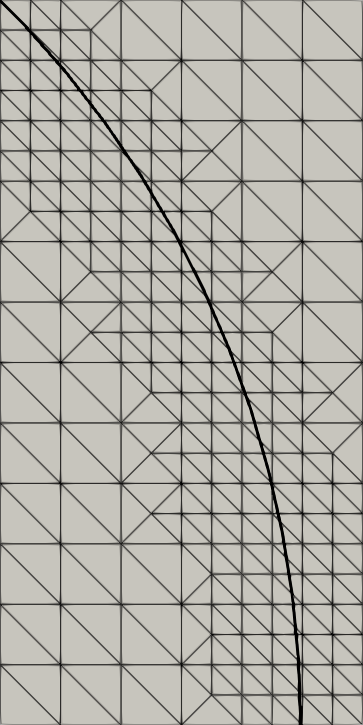
\includegraphics[width=0.19\textwidth]{static/aol-refinedmesh.png}}
\caption{The Python code in Example \ref{example:AOL} solves Example 1 from \cite{AinsworthOdenLee1993}: initial mesh (left), marking by the default-parameter VCD scheme (middle), and the refined mesh (right).  The exact free boundary, unknown to the algorithm, is overlaid in black.}
\label{fig:resultAOL}
\end{figure}

\begin{example} \label{example:hybrid}
The following snippet was used for the left-hand mesh in Figure \ref{fig:threeballmeshes}:
\begin{minted}[linenos, frame=lines]{python}
amr = VIAMR()
fbmark = amr.udomark(uh, psih, n=1)
residual = -div(grad(uh))
imark, _, _ = amr.brinactivemark(uh, psih, residual, theta=0.7)
mark = amr.unionmarks(fbmark, imark)
refinedmesh = amr.refinemarkedelements(mesh, mark)
\end{minted}
Here the $n=1$ case of UDO is used to mark near the free boundary, then the BR error indicator (Section \ref{sec:inactive}), from the element-wise residual, is applied for marking in the inactive set, and finally these marks are unioned.
\end{example}


\section{Results on classical obstacle problems} \label{sec:results}

This section starts with a revised look at how numerical errors should be measured for obstacle problems.  Then we convergence and performance results for our new AMR methods from Sections \ref{sec:inactive} and \ref{sec:viamr} on classical obstacle problems \eqref{eq:classical:vi}.  Section \ref{sec:app} shows results for a more-challenging obstacle problem.

One goal for numerical solutions of obstacle problems is to accurately locate the free boundary and active/inactive sets.  In order to measure the quality of the approximate sets \eqref{eq:fe:sets}, versus the exact sets \eqref{eq:classical:sets}, and determine rates of geometric convergence, the VIAMR library computes a distance between sets.

\begin{definition} \label{def:jaccard}
The \emph{Jaccard distance} \cite{LevandowskyWinter1971} between measurable sets $S,T \subset \Omega$ is
\begin{equation}
d(S,T) = 1 - \frac{|S \cap T|}{|S \cup T|}, \label{eq:jaccard}
\end{equation}
where $|\cdot|$ is Lebesgue measure, with $d(S,T)=0$ by definition if $|S \cup T|=0$.  If $d(S,T)=0$ then $S$ and $T$ geometrically agree up to a set of measure zero.
\end{definition}

We will use Jaccard distance to compare active sets.  A computed active set $A_u^h$ is defined by an element marking (Definition \ref{def:marking}), so we report $d(A_u^h,A_u)$ when $A_u$ is exactly known.  Jaccard distance cannot be used to directly compare free boundary sets, $\Gamma_u^h \approx \Gamma_u$, as these often have measure zero.  Our implementation of \eqref{eq:jaccard} is based on Firedrake's supermesh concept \cite{Farrelletal2009}, so it is computable for sets $S,T$ which are unions of elements from different meshes, and/or for sets defined by algebraic (conditional) expressions in the mesh coordinates.

A second goal for numerical solutions of obstacle problems is to avoid wasted effort in the active set, once the free boundary is well-resolved.  As already discussed, if $\Gamma_u^h \approx \Gamma_u$ is a good approximation then the obstacle data itself, namely $\psi$, should be used to represent the solution in the computed active set $A_u^h$.

\begin{definition} \label{def:preferred}
Suppose the original VI problem \eqref{eq:vi} has exact obstacle $\psi \in \cX\cap C(\bar\Omega)$.  Consider a computed solution $u_h$ to the FE VI problem \eqref{eq:fe:vi}, over a mesh $\cT_h$ on $\Omega$.  Let $A_u^h$ denote the computed active set \eqref{eq:fe:sets}, as a closed union of elements.  We define the \emph{preferred approximation} $\tilde u_h$ as the measurable function
\begin{equation} \label{eq:preferredapprox}
\tilde u_h(x) = \begin{cases} \psi(x), & x\in A_u^h \\ u_h(x), & \text{otherwise.} \end{cases}
\end{equation}
\end{definition}

For a classical obstacle problem \eqref{eq:classical:vi}, the preferred approximation $\tilde u_h$ is in $L^2(\Omega)$.  However, it is generally discontinuous, even when $\cX_h=\CG_k$, and generally $\tilde u_h \notin H^1(\Omega)$.  Importantly, $\tilde u_h$ is defined \emph{without} reference to, or knowledge of, the exact solution to problem \eqref{eq:vi}; only the continuum data $\psi$ is referenced.

We illustrate these principles in the following example.

\begin{example}  \label{example:ball}  Consider the ``ball'' classical obstacle problem shown in Figure \ref{fig:ball} and Figure \ref{fig:activesizes} (middle), which has a known exact solution \cite[Chapter 12]{Bueler2021}.  Algorithms \ref{alg:udo} (UDO) and \ref{alg:vcd} (VCD) were applied to this problem, but combined with inactive-set marking based on the BR error estimator \eqref{eq:brestimator}.  These methods, denoted UDO$+$BR and VCD$+$BR, respectively, avoid refinement in the active set, except near the estimated free boundary.  We also applied mesh adaptation Algorithm \ref{alg:avm} (AVM), setting mesh complexity targets to closely-match the number of elements from the other Algorithms.  Note that AVM refines everywhere, but the meshes are anisotropic, from the Hessian of $u_h$, and free-boundary focussed.

The experiment started from a coarse uniform mesh over the square domain, and applied 11 levels of AMR, so that the number of elements increased by four orders of magnitude.  We also compared uniform refinement.

As shown in Figure \ref{fig:jaccball}, our AMR methods are distinctly superior to uniform refinement when evaluated by active set Jaccard distances $d(A_u^h,A_u)$.  At higher resolutions, all three methods produce distances an order of magnitude smaller than from uniform refinement.  AVM produces the best meshes by this measure, but its runtime is about an order of magnitude higher (not shown).

% see examples/sphere.py and genfigs/ballconv.py for these runs
\begin{figure}[ht]
\centering
\includegraphics[width=0.55\textwidth]{genfigs/jaccball.png}
\caption{Active set Jaccard distances $d(A_u^h,A_u)$.}
\label{fig:jaccball}
\end{figure}

On the other hand, as shown in Figure \ref{fig:ballconv} (left), $L^2$ convergence using the standard error norm $\|u-u_h\|_2$ apparently stagnates for the UDO$+$BR method.  This is entirely due to the contribution from the active set, i.e.~from $|\psi(x) - \psi_h(x)|$ for $x\in A_u^h$, over meshes which have \emph{deliberately} not been refined in $A_u^h$.  If we compute the $L^2$ error relative to the preferred approximation \eqref{eq:preferredapprox}, namely $\|u-\tilde u_h\|_2$, then the convergence is actually slightly better than from uniform refinement, in a per-element sense.  As shown in Figure \ref{fig:ballconv} (right) for the AVM algorithm, because of its active set refinement, the standard ($\|u-u_h\|_2$) and preferred ($\|u-\tilde u_h\|_2$) error norms are comparable. \end{example}

% see examples/sphere.py and genfigs/ballconv.py for these runs
\begin{figure}[ht]
\noindent\mbox{\includegraphics[width=0.49\textwidth]{genfigs/convball_UDO+BR.png} \, \includegraphics[width=0.49\textwidth]{genfigs/convball_AVM.png}}
\caption{Left: $L^2$ norm errors for the UDO$+$BR method, versus uniform refinement.  Results from VCD$+$BR are virtually identical, and not shown.  Right: The same norm errors for the AVM method.}
\label{fig:ballconv}
\end{figure}

To illustrate some additional mesh and performance features of our AMR approaches, we consider three more classical obstacle problem examples.  These do not have known exact solutions.

\begin{example}  \label{example:spiral}  Consider the ``spiral'' example from \cite[subsection 7.1.1]{GraeserKornhuber2009}, shown already in Figure \ref{fig:activesizes} (left).  This example on $\Omega=(-1,1)^2$ has source term $f=0$, homogeneous boundary values $g=0$, and a nontrivial obstacle $\psi$ \cite{GraeserKornhuber2009} in problem \eqref{eq:classical:vi}.  The active set is small in area while the free boundary is long.  A result from applying the UDO$+$BR approach is shown in Figure \ref{fig:spiralmesh}.  (Results from VCD$+$BR and AVM approaches are very similar and not shown.)  At this resolution the free boundary appears to be well-resolved, but in this example there is no performance advantage from avoiding refinement in the small active set. \end{example}

% generated from examples/spiral.py at levels=7
\begin{figure}[ht]
\centering
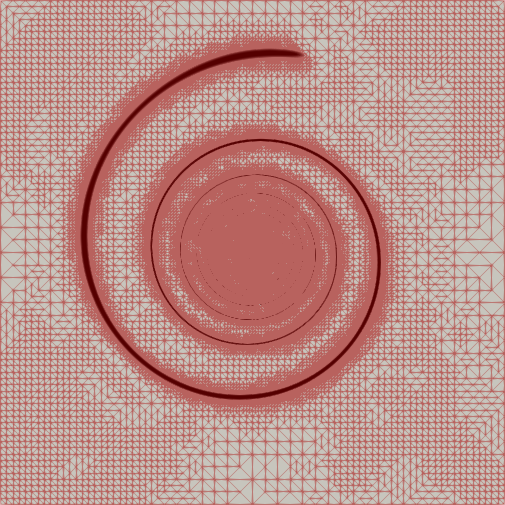
\includegraphics[height=65mm]{static/spiralmesh.png}
\caption{A refined mesh for Example \ref{example:spiral}, with $2\times 10^5$ elements, from seven levels of the UDO$+$BR approach, starting from an initial uniform mesh of 200 elements.  Element diameter (resolution) is about $h=10^{-3}$ along the free boundary.}
\label{fig:spiralmesh}
\end{figure}

\begin{example}  \label{example:blisters}   The example shown in Figure \ref{fig:activesizes} (right), by contrast, has a large active set.  Here $\Omega=(0,1)^2$ and $\psi = g = 0$ in problem \eqref{eq:classical:vi}, but the source term $f$ is a sum of small-variance gaussian peaks against a negative background value; see the code for details.  The blistering property (Appendix \ref{app:blistering}) applies here, so inactive set components must include some area where $f>0$.  The inactive set has six components, but this is only revealed at reasonably high resolution.  Figure \ref{fig:blistersmesh} shows the result of applying the VCD$+$BR method, a mesh with 100 times fewer elements than a uniform mesh of the same free boundary resolution.  Similar to the glacier example in the next Section, in this case the avoidance of active-set refinement gives a distinct performance advantage.  \end{example}

% generated from examples/blisters.py at levels=4
\begin{figure}[ht]
\centering
\mbox{
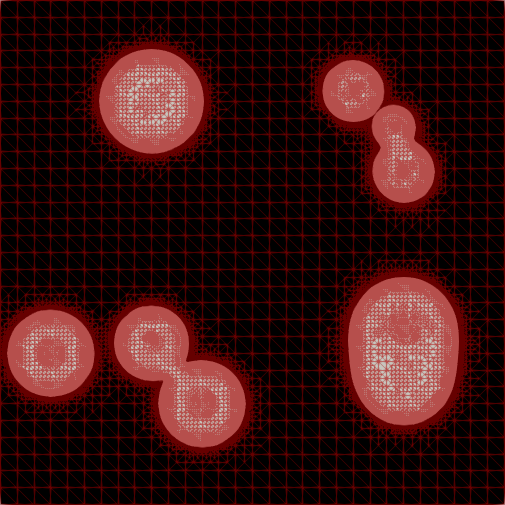
\includegraphics[height=60mm]{static/blistersmesh.png} \qquad
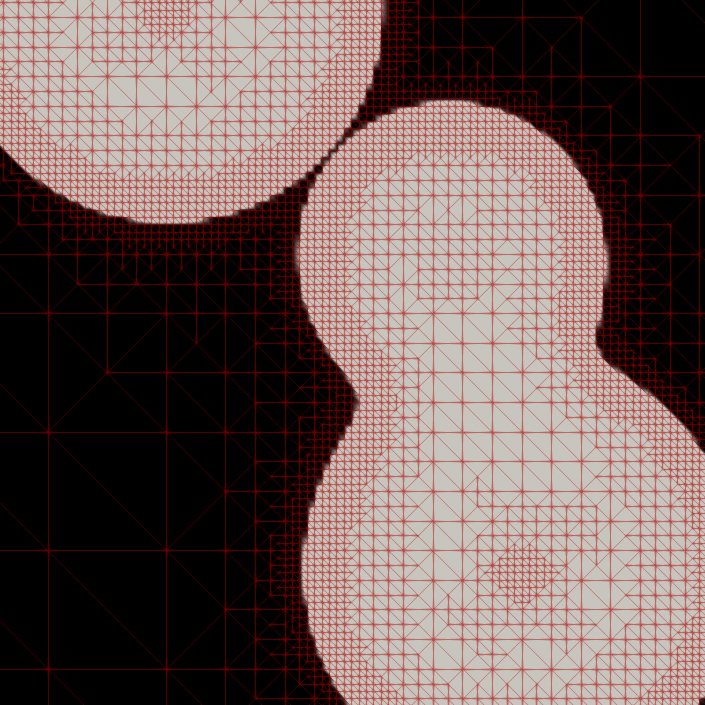
\includegraphics[height=60mm]{static/blisterszoomed.png}
}
\caption{Left: A mesh for Example \ref{example:blisters} of $4.7\times 10^5$ elements, with resolution $h=10^{-3}$ along the free boundary, from four levels of the VCD$+$BR approach, starting from a uniform mesh of 1800 elements.  Right: Zooming-in reveals separation of inactive-set components.}
\label{fig:blistersmesh}
\end{figure}

\begin{example}  \label{example:lshaped}  Our third example is a free-boundary variation of the classic L-shaped Laplace equation problem with an interior corner.  Here the obstacle $\psi$ is the upper unit hemisphere, centered at the origin, and the domain is $\Omega = (-2,5)^2 \setminus S$ where $S$ is a $3\times 3$ square in the lower right corner.  Since $f=0$ and $g=-1$, the Laplace equation is solved in the inactive set, but the Hessian of the solution is singular in the interior corner.  A result from the VCD$+$BR algorithm, starting from a coarse unstructured mesh, is shown  in Figure \ref{fig:lshapedmesh}.  Though the exact free boundary is not known, it has been resolved into a smooth nearly-circular curve, while at the same time there is refinement in the interior corner.  Thus the goals of free-boundary localization and classical PDE AMR are simultaneously addressed. \end{example}

% figure generated from meshfigs/lshaped.pvd
\begin{figure}[ht]
\centering
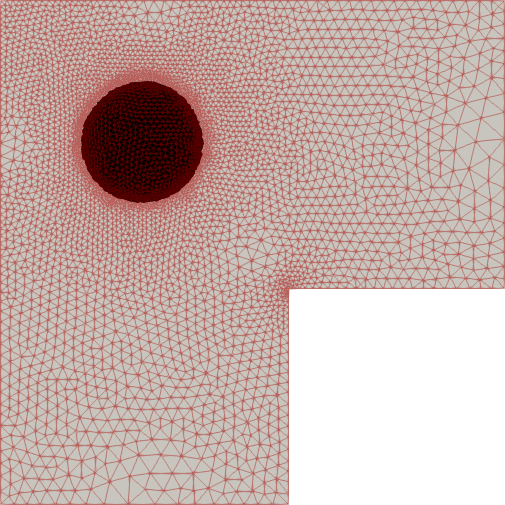
\includegraphics[height=65mm]{static/lshaped.png}
\caption{A refined mesh from five levels of the VCD$+$BR algorithm on Example \ref{example:lshaped}, showing a well-resolved free boundary and refinement in the interior corner.}
\label{fig:lshapedmesh}
\end{figure}


\section{Application to determining glaciated land areas} \label{sec:app}

In this section we apply our AMR techniques to a model for the steady geometry of a glacier, over a given bedrock topography and subject to a given climate.  In particular, this model solves for which land is covered by ice.  Though glacier will cover any land on which snowfall exceeds melt, ice flow expands the ice-covered area out to a free boundary, the glacier margin, which can only be found from conservation equations.  Any fluid layer subject to surface processes which add or remove mass is governed by a similar model \cite{Bueler2021b}.  In these VI problems, which generally are \emph{not} of optimization type, the unknown fluid thickness must be nonnegative, the operator is nonlinear, and the blistering property (Appendix \ref{app:blistering}) applies.

Let $\Omega \subset \RR^2$ be a fixed land region, with bedrock elevation $b=b(x,y) \in C^1(\Omega)$.  Assume there is a surface mass-balance \cite{GreveBlatter2009} function $a:\Omega \times \RR \to \RR$.  This climatic function models the annually-averaged rate of ice accumulation (snow) minus melt and runoff.  If $a$ depends on the surface elevation $s$ then we suppose that $a(x,y,s)\in L^\infty(\Omega)$ for any $s=s(x,y) \in L^\infty(\Omega)$, and additionally that $a$ is Lipschitz continuous in $s$.

We use an ice flow approximation called the \emph{shallow ice approximation} \cite{GreveBlatter2009}, derived by a thin-layer argument from mass and momentum conservation, in its simplest isothermal and non-sliding case.  Applying the standard exponent for the shear-thinning flow law of ice \cite{GreveBlatter2009}, we have a VI for admissible transformed ice thickness functions $u \in \cK = \{u \in \cX\,:\,u\ge 0 \text{ and } u|_{\partial\Omega}=0\}$, in the Banach space $\cX = W^{1,4}(\Omega)$ \cite{JouvetBueler2012}.  The thickness itself is $H=u^{3/8}$, while the surface elevation is $s=H+b=u^{3/8}+b$.  The model is a VI based upon a ``tilted'' variation of the $p$-Laplacian operator \cite{JouvetBueler2012}:
\begin{equation}
\int_\Omega \Gamma |\grad u + \bm{\beta}(u)|^2 (\grad u + \bm{\beta}(u)) \cdot \grad (v-u) - \tilde a(u) (v-u)\,dx \ge 0 \label{eq:sia:vi}
\end{equation}
for all $v \in \cK$.  Here $\Gamma>0$ is an ice softness constant, $\bm{\beta}(u)=\frac{8}{3} u^{5/8} \grad b$ is a nonlinear multiple of the bed gradient, and $\tilde a(u)=a(x,y,u^{3/8}+b(x,y))$ denotes the surface mass balance (with $x,y$ dependence suppressed).  When $\grad b=0$, \eqref{eq:sia:vi} defines a nonlinear operator $F(v)[w]$ which is $4$-coercive \cite{JouvetBueler2012}; recall definition \eqref{eq:coercive}.  If $a$ has no $s$ dependence then one may treat it as the source term, and write ``$F(u)[v-u]\ge\ell[v-u]$'' as in \eqref{eq:vi}, but otherwise we simply set $\ell=0$ in \eqref{eq:vi}.

Regarding the mathematical theory of \eqref{eq:sia:vi}, existence holds for any $b$ when $a$ is independent of $s$ \cite{JouvetBueler2012}.  Simple cases of \emph{non}-existence are known wherein $a$ depends on $s$ \cite{Jouvetetal2011}, but our examples below have slow increase of snowfall with elevation \cite{GreveBlatter2009}, avoiding the issue.  The strong-form interior condition of \eqref{eq:sia:vi} is a conservation equation:
\begin{equation}
\Div \bq = \tilde a \text{ over } I_u, \quad \text{where } \bq = - \Gamma |\grad u + \bm{\beta}(u)|^2 (\grad u + \bm{\beta}(u)).
\label{eq:sia:interior}
\end{equation}
At the free boundary (glacier margin) the solution $u$, the solution gradient $|\grad u|$, and the flux $\bq$ all go to zero.  On the other hand, observations confirm that the gradient of a glacier's surface has large magnitude as one approaches the margin from the ice side, a property which emerges from \eqref{eq:sia:vi} when one differentiates the associated surface elevation $s=u^{3/8} + b$, and in fact generally $|\grad s| \to \infty$ at the glacier margin.

We apply a conforming, continuous, piecewise-linear FE method \eqref{eq:fe:vi}, over unstructured triangulations.  The FE problem is either solved directly by the same VI-adapted Newton solver (\texttt{vinewtonrsls} in PETSc \cite{petsc-user-ref}) used in Section \ref{sec:results}, or with an added outer Picard-type iteration over the tilt $\bm{\beta}(u)$ \cite{JouvetBueler2012} and source $\tilde a(u)$, with Newton as the inner iteration.  The linear Newton steps are solved directly.  Very similar results are obtained when both converge, but the Picard-based solver is more robust when $|\grad b|$ is large or $\tilde a$ depends on $u$.

We consider two particular problems, each over a square domain $\Omega=(0,L)^2$, $L=1800$ kilometers.  The first ``dome'' problem has a flat bed, elevation-independent source, and a known exact solution \cite{Bueler2016}; this is used for verification and to compare AMR algorithms.  The second ``realistic'' problem has a bumpy bed and an elevation-dependent surface mass balance function.

\begin{example} \label{example:dome}
The dome problem was solved with 13 levels of refinement from an initial, uniform $h_0=360$ kilometer mesh to a final mesh with glacier margin resolution of $h_{13}\approx 30$ meters.  Both UDO and VCD methods (Section \ref{sec:viamr}) were applied, with GR marking in the inactive set (Section \ref{sec:inactive}).  Because the obstacle is $\psi=0$, the preferred and standard numerical solutions agree (see \eqref{eq:preferredapprox}), and numerical errors can be computed in the usual manner.  Figure \ref{fig:domenormresults} shows relative $H^1$ errors in the solution ($\|u-u_h\|_{H^1}/\|u\|_{H^1}$) and absolute $L^\infty$ errors in the corresponding ice thickness ($\|H-H_h\|_{L^\infty}$), versus number of elements.  The latter errors are much more responsive to AMR because the physical ice thickness gradient is singular at the free boundary, so (lateral) margin location error is effectively being measured.  Figure \ref{fig:domeradiusresults} shows the maximum radial error for the numerical margin, illustrating the free-boundary localization for the same runs.  We see that AMR methods are much more efficient for this purpose, compared to uniform refinement, similarly to the ball problem result in Section \ref{sec:results}, and again that the UDO and VCD variants perform very similarly.
\end{example}

% see examples/glacier/README.md for these runs
\begin{figure}[ht]
\noindent\mbox{\includegraphics[width=0.49\textwidth]{genfigs/uerrh1.png} \, \includegraphics[width=0.49\textwidth]{genfigs/herrinf.png}}
\caption{Left: $H^1$ norm errors in $u$ are comparable for AMR and uniform refinement, in a per-element sense.  Right: AMR is effective for the maximum thickness error.}
\label{fig:domenormresults}
\end{figure}

\begin{figure}[ht]
\centering
\includegraphics[width=0.51\textwidth]{genfigs/drmax.png}
\caption{AMR generates accurate free boundary locations.  To achieve tens of meters accuracy, as here, uniform refinement would use orders of magnitude more elements.}
\label{fig:domeradiusresults}
\end{figure}

\begin{example} \label{example:realistic}
The next example is more realistic.  It uses a bumpy bedrock topography $b(x,y)$, a finite sum of sinusoids \cite[Example 8.4]{BuelerFarrell2024}, and a surface mass balance function $a(s)$ which depends only on surface elevation.\footnote{For detailed formulas see the source code in \href{https://github.com/StefanoFochesatto/VI-AMR/examples/glacier/}{{\scriptsize \texttt{github.com/StefanoFochesatto/VI-AMR/examples/glacier/}}}.}  An important parameter in the formula for $a(s)$ is the equilibrium line altitude (ELA) \cite{GreveBlatter2009}, with $a>0$ above this altitude and $a< 0$ below.  Figure \ref{fig:transect} shows the topography along a transect $x=\hat x$ (red line in Figure \ref{fig:glacier}), with three ELA values $s_0$ superimposed.  Bedrock above the ELA will certainly be glacier-covered, but snowfall occurs on a larger solution-dependent set, namely $S=\{(x,y)\,:\,u(x,y)^{3/8} + b(x,y) > s_0\}$, and glaciation extends beyond $S$ because of flow: $I_u \supset S$.  The difficult nonlinearities in model \eqref{eq:sia:vi} include this elevation-dependent surface mass balance, but also the $u^{5/8}$ dependence in the tilt $\bm{\beta}(u)$.  Among the other effects of the latter nonlinearity is the tendency of ice to pool in bedrock elevation lows.

\begin{figure}[ht]
\centering
\medskip

\includegraphics[width=0.96\textwidth]{genfigs/transect.png}
\caption{Bedrock elevation (solid) along a transect (red in Figure \ref{fig:glacier}, left), with three ELA levels (dashed).}
\label{fig:transect}
\end{figure}

Our primary goals in this example are to generate an accurate map of glaciation, i.e.~of the inactive set $I_u$, to estimate the location of the glacier margin ($\Gamma_u$), and to compute the ice volume $V=\int_\Omega u^{3/8}\,dx\,dy$.  Note that the number of connected components of $I_u$, i.e.~the number of glaciers, is also a model output.

We applied UDO (Algorithm \ref{alg:udo}), with $n=2$ levels, and GR marking in the inactive set.  A minimum element diameter $\hmin=500$ meters (Section \ref{sec:viamr}) was set, with the resulting meshes having about 300 meter resolution along most of the glacier margin.  For ELA values $s_0=1000,800,600$ meters, the resulting surface elevation maps are shown in Figure \ref{fig:glacier}.  The varying ice volumes, $1.1\times 10^5$, $5.6\times 10^5$, and $8.9\times 10^5$ cubic kilometers, respectively, reflect the strong climate (ELA) sensitivity  of realistic glacier models \cite{GreveBlatter2009}.\footnote{Compare the volume of the present-day Greenland ice sheet at $2.9\times 10^6$ cubic kilometers.}

% see examples/glacier/{steady.py|caps.sh} for information about these runs
\begin{figure}[ht]
\centering

\mbox{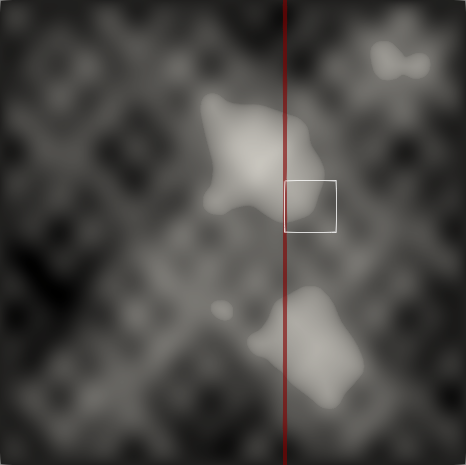
\includegraphics[width=0.32\textwidth]{static/glacier/surf1000.png} \,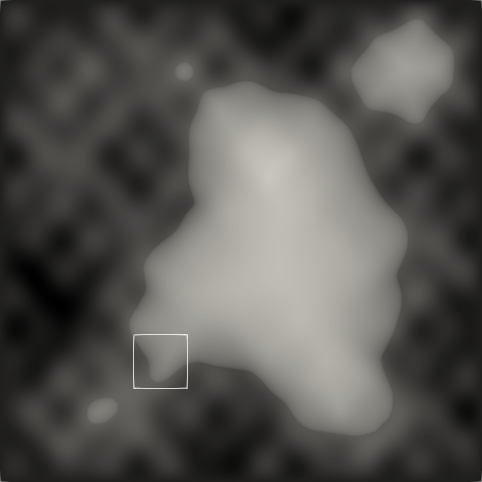
\includegraphics[width=0.32\textwidth]{static/glacier/surf800.png} \,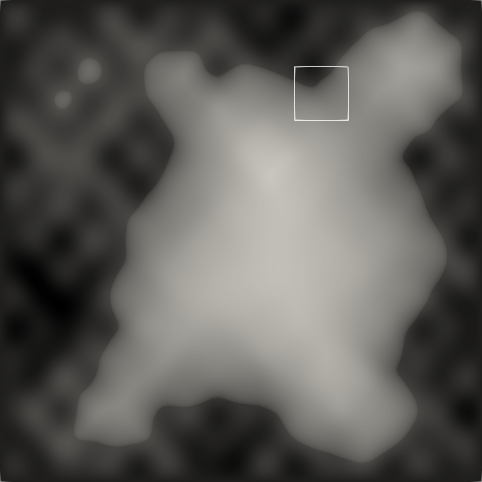
\includegraphics[width=0.32\textwidth]{static/glacier/surf600.png}}
\caption{Glacier surface elevation (grayscale) for ELA of 1000 meters (left), 800 meters (middle), and 600 meters (right).  Inset boxes are 200 km across; see Figure \ref{fig:insetmeshes}.}
\label{fig:glacier}
\end{figure}

Figure \ref{fig:insetmeshes} shows details of the resulting meshes along sample portions of the glacier margins.  It is key to observe that under the UDO$+$GR AMR approach the mesh was \emph{not} refined in the vast majority of the active set, and this represents a significant efficiency.  That is, we did not waste computational effort (e.g.~elements) on modeling ice which turned out to not be present.  Also we observe that this highly-nonlinear problem causes AMR to work hard to pin down the glacier margin, as only once the inactive side of the margin is resolved at high resolution will its location stabilize.
\begin{figure}[ht]
\centering
\mbox{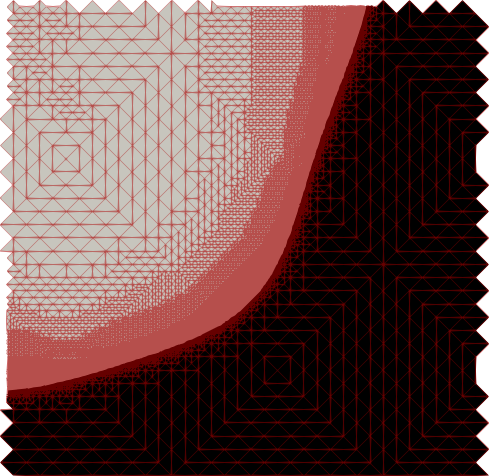
\includegraphics[width=0.32\textwidth]{static/glacier/sub1000.png} \,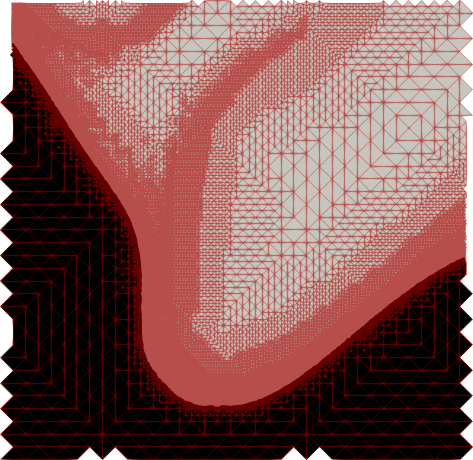
\includegraphics[width=0.32\textwidth]{static/glacier/sub800.png} \,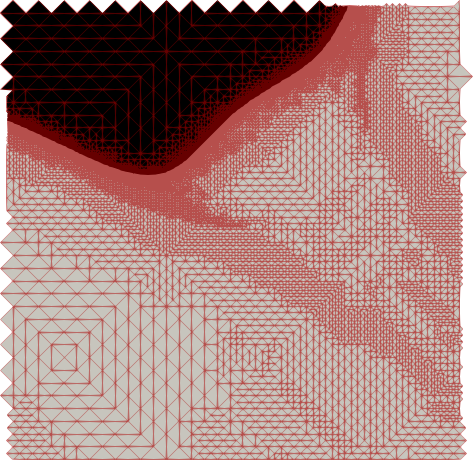
\includegraphics[width=0.32\textwidth]{static/glacier/sub600.png}}
\caption{Details of refined meshes (red) along glacier margins, from the inset boxes in Figure \ref{fig:glacier}, for the same ELA values.  The dark areas are coarsely-meshed ice-free areas, i.e.~active sets.}
\label{fig:insetmeshes}
\end{figure}
\end{example}


\section{Discussion and conclusion} \label{sec:conclusion}

FIXME \emph{Grid Sequencing + AMR targeting the free boundary} is the iterative process for how we are converging to the FB.  The bulk of vinewton iterations are coming from stabilizing the initial iterate's FB and thereafter Grid Sequencing is allowing us to make small adjustments as we refine.  the grid sequencing works best on hierarchal meshes, while with metric method the "grid sequencing" is done through cross-mesh interpolation.

FIXME We have no quantitative theory (norm bounds) telling us how the two strategies interact.  We are applying two different, well-defined, marking strategies:
\begin{enumerate}
\item assuming $u_h$ gives an estimate of the free boundary, mark nearby elements on both sides of the free boundary
\item assuming $u_h$ gives an estimate of the inactive set, mark in this approximate inactive set according to PDE principles
\end{enumerate}
Note that i) has nothing directly to do with the regularity (or residual) in $u_h$.  Regardless of the smoothness of $u_h$ near the free boundary, or the magnitude of the residual from $u_h$, we want to mark near the free boundary.

FIXME VI solver performance can be substantially improved by combining the AMR meshing strategies here with a multilevel approach.  The solver in \cite{BuelerFarrell2024}, for example, uses coarse meshes to make large geometrical corrections in the free boundary.  This path, which promises highly-scalable solutions of obstacle problems, is for future research.

%\section*{Acknowledgements}

%\section*{Notes on contributor(s)}
%An unnumbered Section, e.g.\ \verb"\section*{Notes on contributors}", may be included \emph{in the non-anonymous version} if required. A photograph may be added if requested.


\bibliographystyle{tfs}
\bibliography{viamr}


%Any appendices should be placed after the list of references, beginning with the command \verb"\appendix" followed by the command \verb"\section" for each appendix title, e.g.
\appendix
\section{Unilateral obstacle problems with the blistering property} \label{app:blistering}

In classical obstacle problem \eqref{eq:classical:vi} an upward force $f(x)>0$ may generally occur in the active set $A_u$.  Physically speaking, an upward force may be insufficient to lift $u$ off a concave obstacle $\psi$.  However, in certain problems this situation cannot occur.  The hypotheses of Lemma \ref{lem:blister} hold for porous dam saturation free-boundary problems \cite[for example]{AinsworthOdenLee1993} and the glacier problem in Section \ref{sec:app}.

\begin{lemma} \label{lem:blister}
Suppose that $\psi=0$ and $\ell[v] = \int_\Omega fv\,dx$ for $f\in L^2(\Omega)$.  Suppose also that the operator $F$ is given by measurable densities: $F(w)[v]=\int_\Omega \phi(w(x),\grad w(x)) v(x) + \Phi(w(x),\grad w(x)) \cdot \grad v(x)\,dx$.  Assume the densities satisfy $\phi(0,0)=0$ and $\Phi(0,0)=0$.  Then for $u$ solving \eqref{eq:vi}, $f\le 0$ a.e.~in $A_u$.
\end{lemma}

\begin{proof}
Let $S\subset A_u$ be a Borel set, and denote its indicator function by $\chi_S \in L^\infty(\Omega)$.  By a density argument and the assumptions on $\phi$ and $\Phi$, the operator value $F(u)[\chi_S]$ is well-defined, \emph{and zero}, because $S$ is in the active set.  Thus by Lemma \ref{lem:measure},
\begin{equation*}
0 \le d\mu_u(S) = F(u)[\chi_S]-\ell[\chi_S] = 0 - \ell[\chi_S] = -\int_S f\,dx.
\end{equation*}
This shows $f\le 0$ a.e.~(with respect to Lebesgue measure).
\end{proof}

\begin{definition}
For a unilateral obstacle problem \eqref{eq:vi} with source term $\ell[v] = \int_\Omega fv\,dx$, $f\in C(\bar \Omega)$, we say that \emph{blistering property} holds if $A_u \subset \{x \in \Omega\, :\, f(x)\le 0\}$ \cite{JouvetBueler2012}, that is, if the conclusion of Lemma \ref{lem:blister} holds.
\end{definition}

To explain the language, if $f(x)>0$ for some $x\in\Omega$ then, assuming this property, the inactive set $I_u$ must be non-empty, and $x\in I_u$.  That is, even a small upward force ``blisters'' the membrane off the obstacle.

Any classical problem \eqref{eq:classical:vi} with a smooth obstacle $\psi\in C^2(\bar\Omega)$ can be transformed into one with the blistering property.  Let $\tilde v=v-\psi$, thus $\tilde\cK = \{\tilde v\in\cX\,:\,\tilde v\ge 0 \text{ and } \tilde v|_{\partial\Omega}=g-\psi|_{\partial\Omega}\}$.  Integration-by-parts shows \eqref{eq:classical:vi} is equivalent to finding $\tilde u = u -\psi \in \tilde \cK$ so that
\begin{equation} \label{eq:classical:vi:blister}
\int_\Omega \nabla \tilde u \cdot \nabla(\tilde v - \tilde u) \ge \int_\Omega \left(f+\grad^2\psi\right)(\tilde v - \tilde u) \quad \text{ for all } \tilde v \in \tilde \cK.
\end{equation}
For VI problem \eqref{eq:classical:vi:blister}, if $x\in A_{\tilde u} = \{\tilde u(x)=0\}$ then $\tilde f(x)= f(x)+\grad^2\psi(x)\le 0$.

For blistering-property problems, AMR costs can be reduced by avoiding refinement in the computed active sets.  From a computed solution $u_h$, one starts by identifying the elements $K\in \cT_h$ in the computed active set $A_u^h$.  (In our implementation we require that every node in the closure of $K$ is active, according to some tolerance.)  To identify $K$ where no refinement would be beneficial, the degenerate case must be excluded, so we require $K \subset \Omega_- = \{x\in \Omega\,:\,f(x) < 0\}$; this uses only the data of the problem.  If later refinements move the free boundary to be incident to $K$ then refinement of $K$ becomes appropriate.

In summary, if a problem has the blistering property, and if $f < 0$ on a currently-active element $K$, then $K$ can likely remain unrefined without affecting solution accuracy.  Section \ref{sec:viamr} techniques are designed to mark active-set elements which are near $\Gamma_u^h$, in a geometrical sense, for refinement.  Refinement in the inactive set, e.g.~based on indicators from Section \ref{sec:inactive}, is also necessary to give accuracy $\Gamma_u^h \approx \Gamma_u$.

\end{document}
